\documentclass[a4paper,12pt]{article}

%%%%%%%%%%%%%%%%%%%%
%%%%  PREAMBLE  %%%%
%%%%%%%%%%%%%%%%%%%%

\usepackage[T1]{fontenc}
\usepackage[utf8]{inputenc}

\usepackage[english,italian]{babel}

\usepackage{hyperref}
\hypersetup{hidelinks}

\usepackage[margin=2.5cm]{geometry}
\usepackage{minipage-marginpar}
\usepackage{fancyhdr}
\usepackage[bottom]{footmisc}
\usepackage{lastpage}

\usepackage{enumitem}
\usepackage{tabularx}

\usepackage{graphicx}

\setlength{\parindent}{0em}
\setlength{\parskip}{1em}

\fancyhead[L]{\leftmark}
\fancyhead[R]{\shortstack[r]{Versione documento: 0.01 \\ Gruppo: T27}}

\fancyfoot[C]{}
\fancyfoot[R]{\thepage/\pageref{LastPage}}

\renewcommand{\headrulewidth}{2pt}
\renewcommand{\headruleskip}{3pt}
\setlength{\headheight}{30pt}

\renewcommand{\footrulewidth}{2pt}

\setlist[itemize]{itemsep=0.25em,topsep=0pt}
\setlist[enumerate]{itemsep=0.25em,topsep=0pt,align=left}

%%%%%%%%%%%%%%%%%%%%
%%%%  DOCUMENT  %%%%
%%%%%%%%%%%%%%%%%%%%

\title{Web Music Player}
\author{Gruppo T27}

\begin{document}

\pagestyle{empty}

\begin{center}

    \vspace{2 cm}

    \begin{tabular*}{\textwidth}{ c @{\extracolsep{\fill}} c }
        
\includegraphics[width=0.3\textwidth]{marchio_unitrento.pdf} & \shortstack{\Large{Dipartimento di Ingegneria} \\ \Large{e Scienza dell'Informazione}}
    \end{tabular*}

    \vspace{2 cm} 
  
    \LARGE{Ingegneria del software\\}
  
    \vspace{1.5 cm} 
    \Large\textsc{Documento dei requisiti\\} 
    \Large\textsc{Versione: 0.01\\} 
    \vspace{2 cm} 
    \Huge\textsc{Web Music Player\\}
    \Large{\it{Gruppo T27}}
  
    \vspace{2 cm} 
  
    \Large{Anno accademico 2022/2023}
\end{center}

\newpage
\tableofcontents

\pagestyle{fancy}

\newpage
\section{Scopo del documento}

Il presente documento riporta l’analisi dei requisiti di sistema del progetto Web Music Player. Lo scopo di questo di questo documento è quello di:
\begin{itemize}
    \item descrivere gli obiettivi funzionali;
    \item elencare i requisiti non funzionali;
    \item mostrare le interazioni del progetti con altri sistemi;
    \item mostrare le componenti interne del sistema.
\end{itemize}

\newpage
\section{Requisiti funzionali}

Andiamo a descrivere nel dettaglio i requisiti funzionali del sistema. Per fare ciò, sfruttiamo gli use-case diagram, un utile strumento di visualizzazione. Ciascuno use-case diagram sarà accompagnato da una descrizione; questa può essere testuale o tramite un ulteriore diagramma.

\subsection*{RF1 Registrazione}

\begin{figure}[htp]
    \centering
    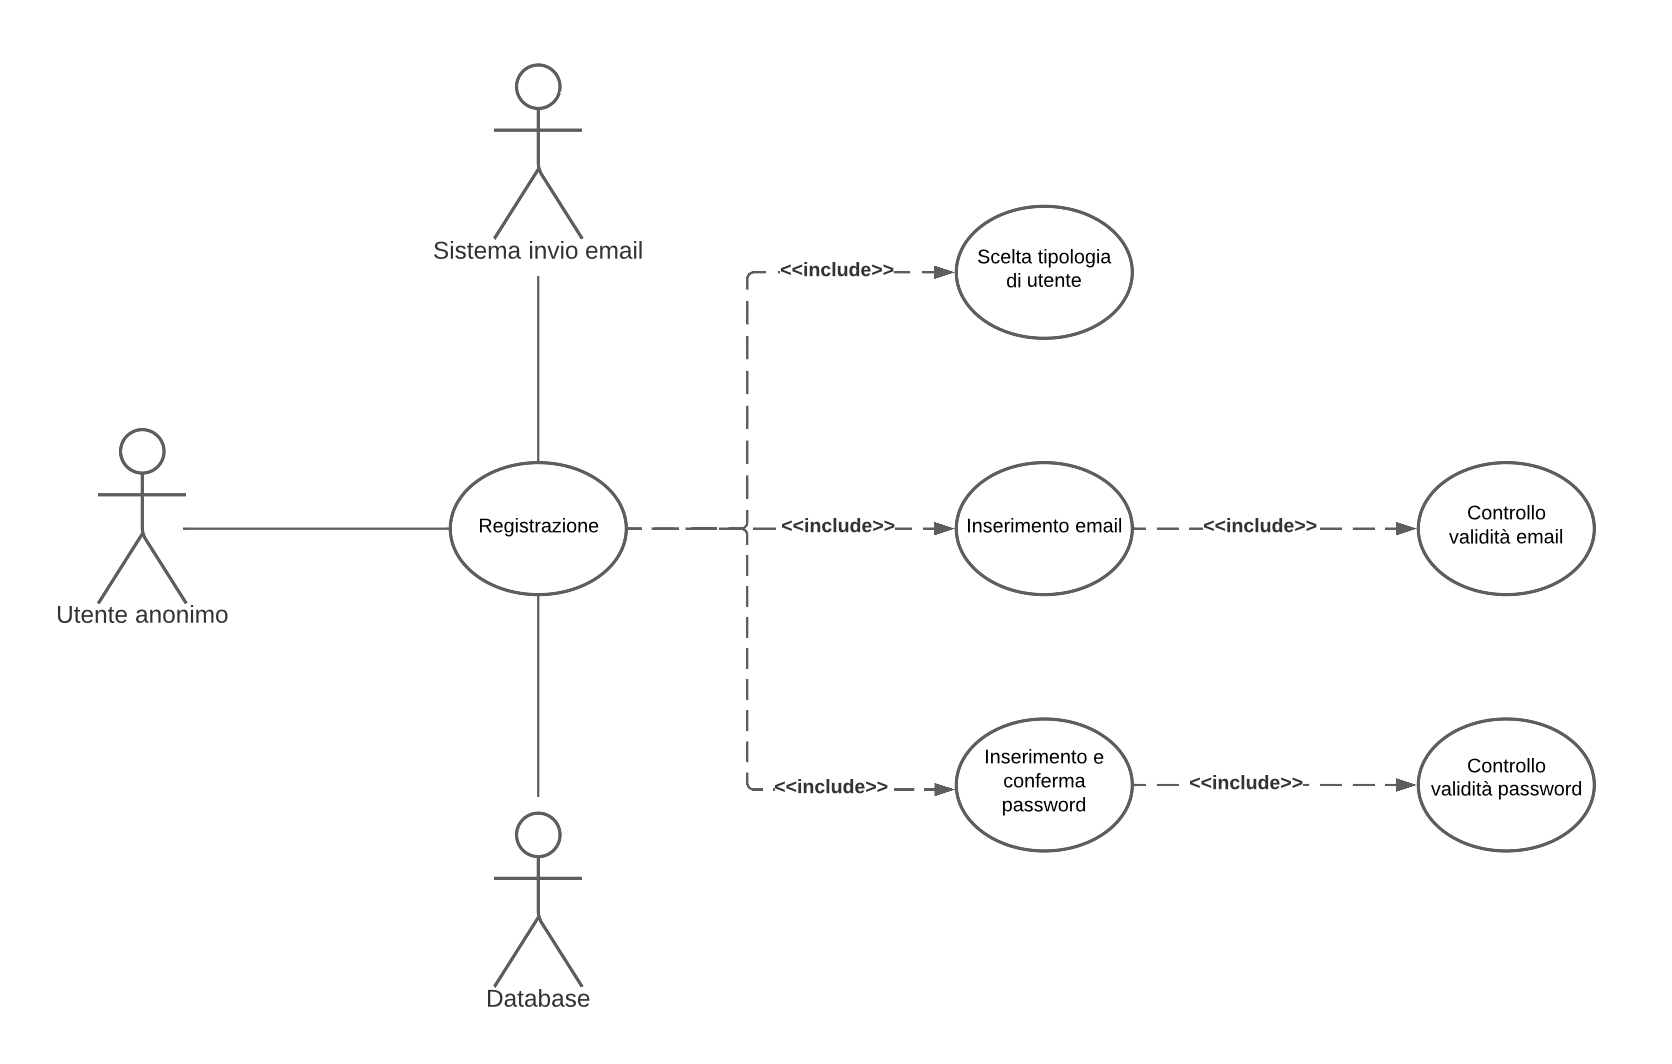
\includegraphics[width=0.75\textwidth]{diagrams/use-case-1.png}
\end{figure}

Per descrivere questo use-case, facciamo uso di un diagramma delle attività:

\begin{figure}[htp]
    \centering
    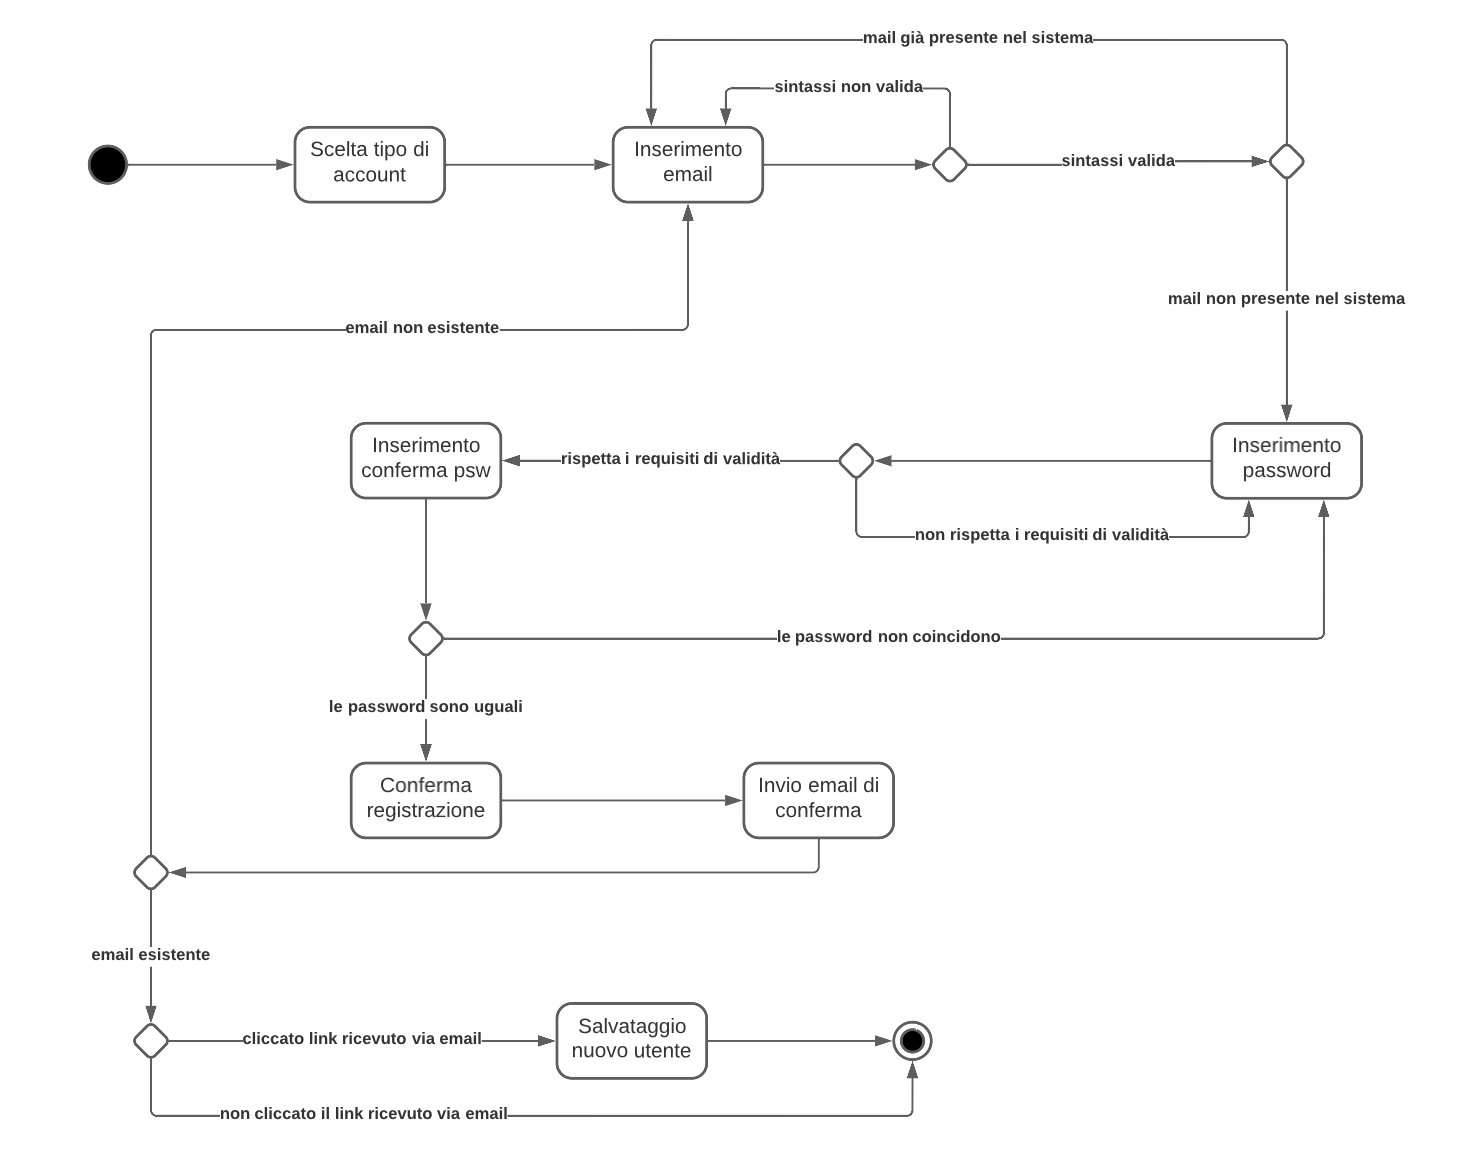
\includegraphics[width=0.75\textwidth]{diagrams/activity-1.png}
\end{figure}

\newpage

\subsection*{RF2 Pagamento}

\begin{figure}[htp]
    \centering
    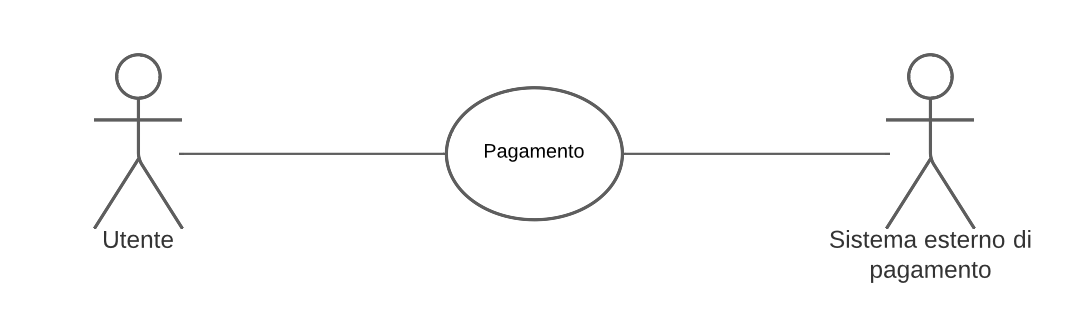
\includegraphics[width=0.75\textwidth]{diagrams/use-case-2.png}
\end{figure}

\textbf{Descrizione:} l'utente paga il servizio tramite un sistema esterno. 

\vspace{1em}
\subsection*{RF3 Login}

\begin{figure}[htp]
    \centering
    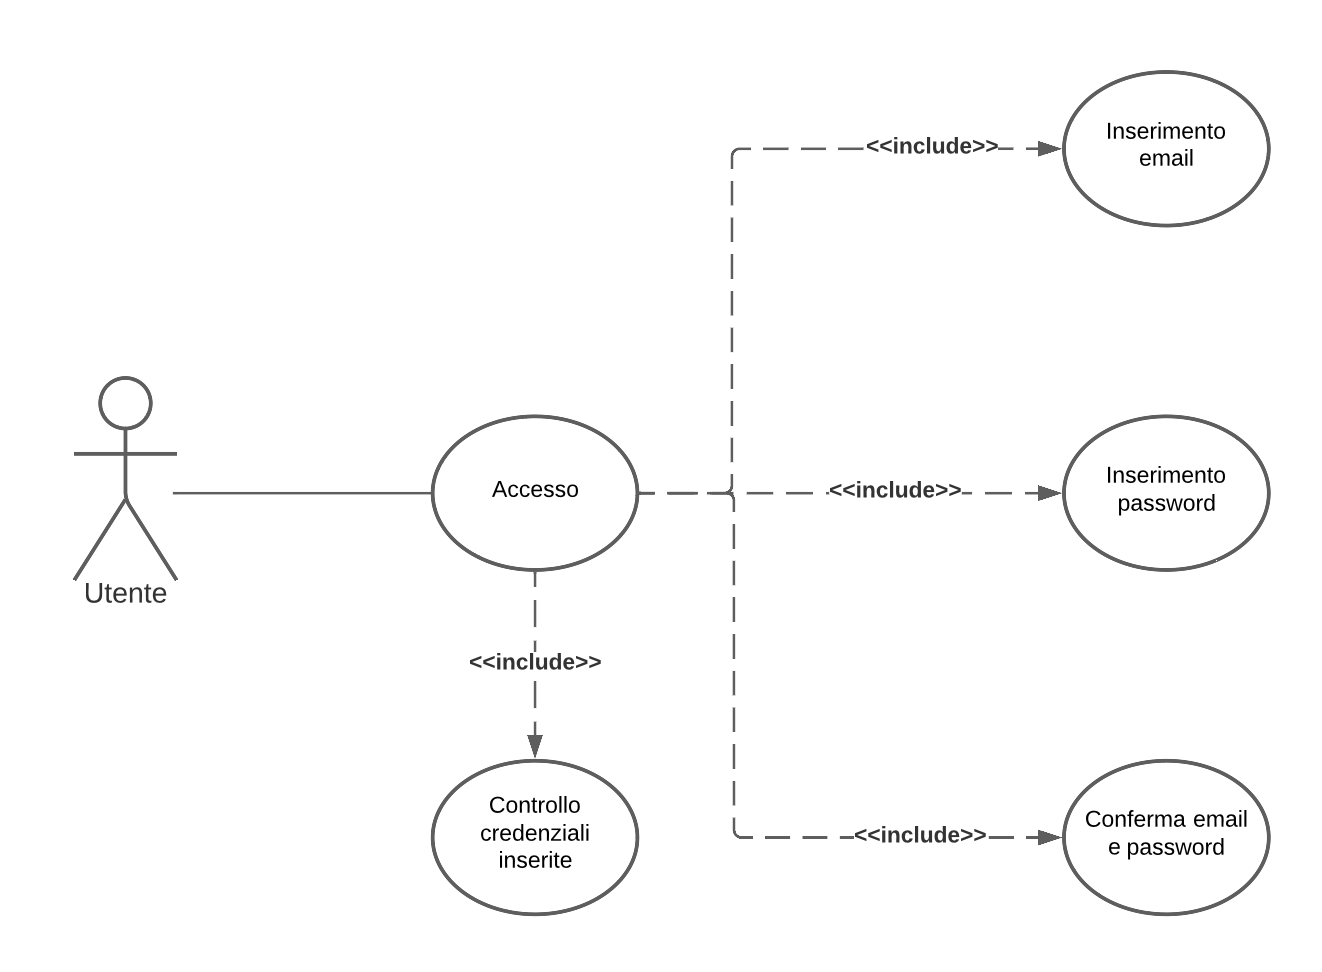
\includegraphics[width=0.75\textwidth]{diagrams/use-case-3.png}
\end{figure}

\textbf{Descrizione:} questo use-case descrivere l’accesso al sito per un utente già registrato.

\textbf{Passi:}
\begin{enumerate}
    \item L’utente inserisce la sua mail 
    \item L’utente inserisce la password associata al suo account 
    \item L’utente conferma la mail e la password inserite
    \item Il sistema verifica la correttezza di mail e password \textbf{[exception 1]}
    \item L’utente entra nel sito
\end{enumerate}

\textbf{[exception 1]} Nel caso in cui l’email e/o la password siano errati viene esposto un messaggio di errore: “email e/o password errati”.

\newpage

\subsection*{RF4 Recupero password}

\begin{figure}[htp]
    \centering
    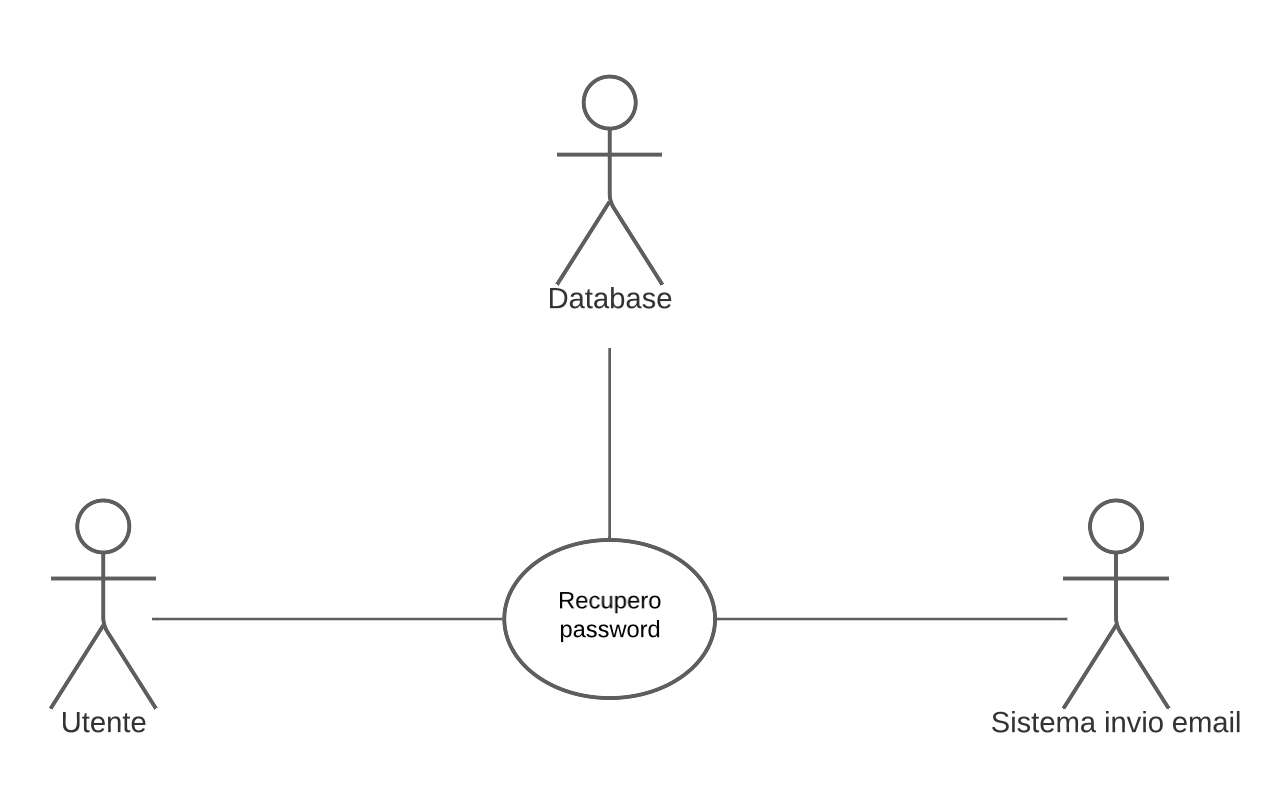
\includegraphics[width=0.75\textwidth]{diagrams/use-case-4.png}
\end{figure}

Per descrivere questo use-case, facciamo uso di un diagramma delle attività:

\begin{figure}[htp]
    \centering
    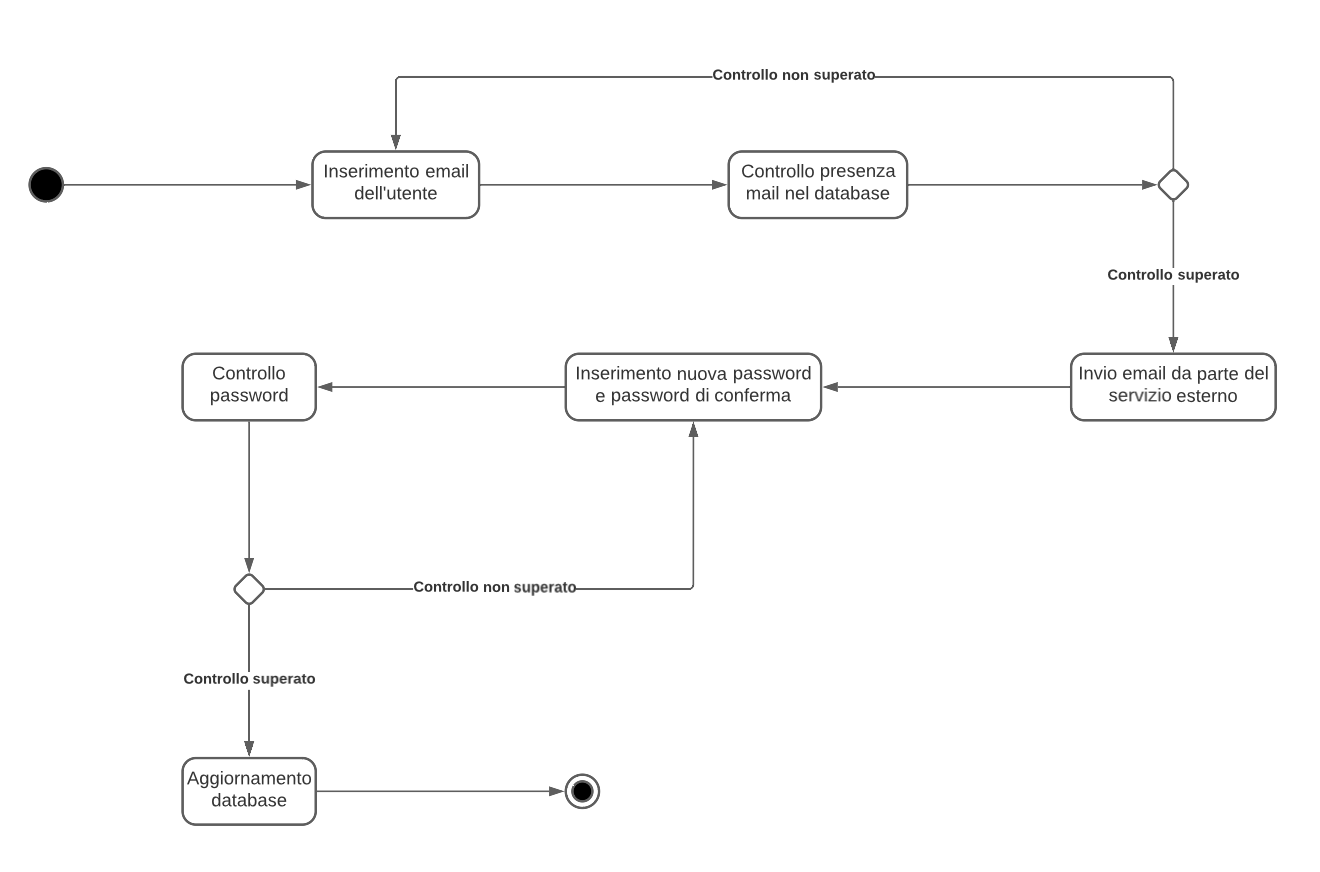
\includegraphics[width=0.75\textwidth]{diagrams/activity-4.png}
\end{figure}

\subsection*{RF 5-13}

\begin{figure}[htp]
    \centering
    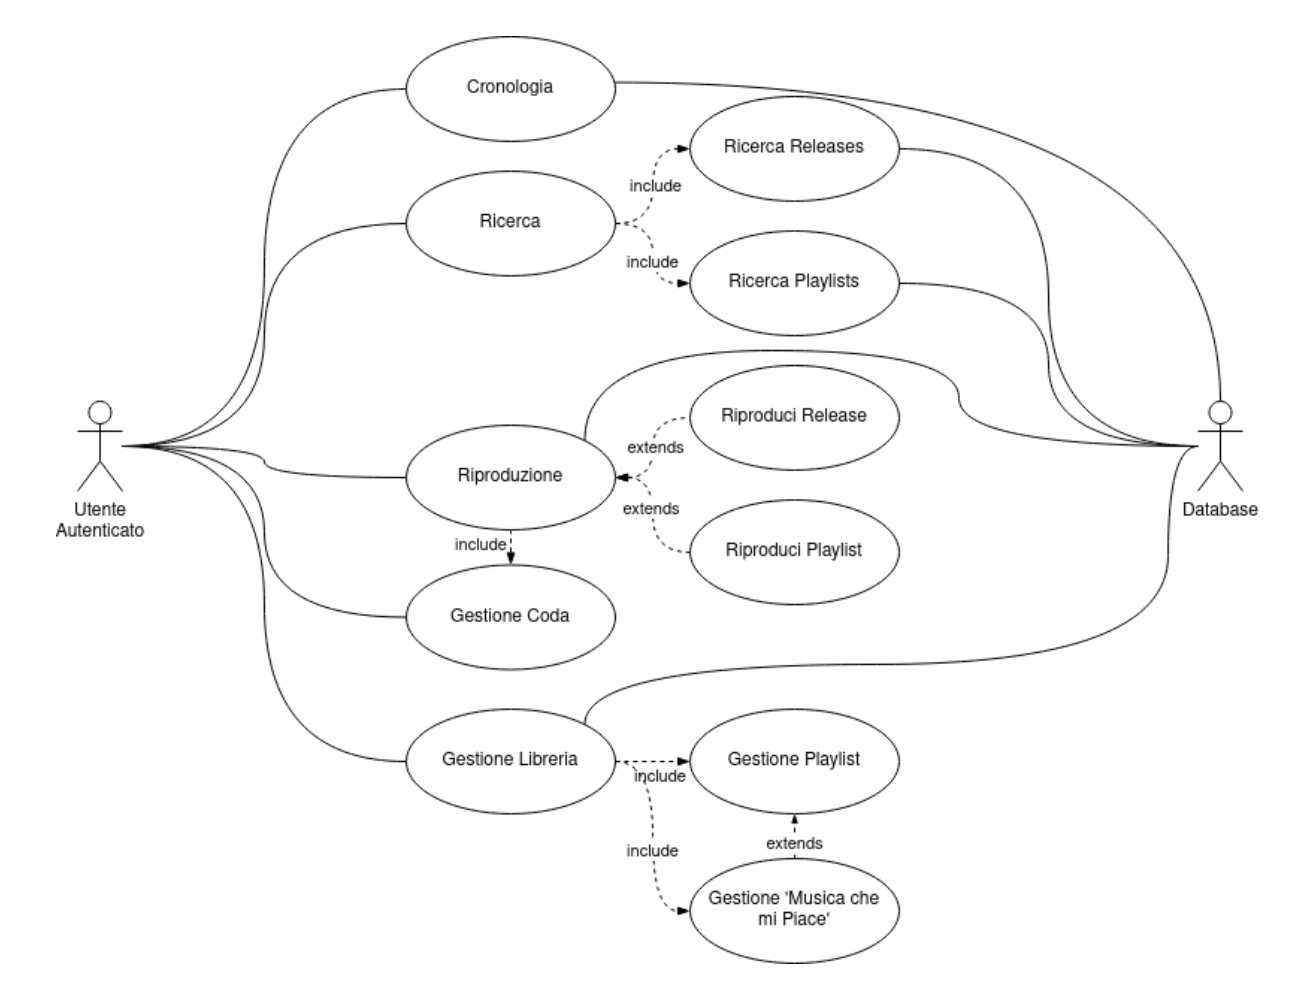
\includegraphics[width=0.75\textwidth]{diagrams/use-case-5-6-7-8-9-10-11-12-13.png}
\end{figure}

\subsubsection*{RF5 Ricerca}
\textbf{Descrizione:} l’utente deve poter ricercare releases, artisti e playlists. \newline
\textbf{Passi:}
\begin{enumerate}
    \item L’utente inserisce del testo nella barra di ricerca
    \item Il sistema ricerca in modo approssimato tra le releases sulla piattaforma, i creator registrati e le playlist create e restituisce una lista di risultati, ordinati in base a quello più vicino alla query
\end{enumerate}

\subsubsection*{RF 6 Riproduzione}

\textbf{Descrizione:} l’utente deve poter riprodurre una release o una playlist a partire da un brano e avere quelli successivi automaticamente messi nella coda di riproduzione nel corretto ordine. \newline
\textbf{Passi:}
\begin{enumerate}
    \item L’utente preme sull’apposito pulsante per iniziare la riproduzione del brano \textbf{[extension 1]}
    \item Il client dialoga col sistema per iniziare lo stream
    \item Il client elabora lo stream seguendo la specifica del DRM
\end{enumerate}
\textbf{[extension 1]} Se il brano si trova in una playlist e non è l’ultimo, il client si dovrà premurare di aggiungere anche i brani che vengono dopo alla coda nello stesso ordine in cui appaiono nella playlist. Similmente, se il brano viene riprodotto come parte di una release e non è l’ultimo, il client dovrà aggiungere alla coda i brani che succedono quello riprodotto nell’ordine corretto.

\subsubsection*{RF 7 Coda}

\textbf{Descrizione:} l’utente deve poter gestire la propria coda di riproduzione (riordinarla, rimuovervi brani e aggiungerne) e il client deve seguire la coda per sapere l’ordine in cui vanno riprodotte le canzoni. \newline
\textbf{Passi:}
\begin{enumerate}
    \item L’utente, attraverso appositi pulsanti, è in grado di riordinare, rimuovere e aggiungere brani alla coda
    \item Il client, unico posto dove la coda è mantenuta, deve salvare ogni modifica
    \item Una volta che la riproduzione del brano corrente è terminata, la coda va utilizzata per trovare il prossimo brano da riprodurre
\end{enumerate}

\subsubsection*{RF 8 Libreria}

\textbf{Descrizione:} l’utente deve poter vedere le proprie playlists e la musica che ha salvato.

\subsubsection*{RF 9 Preferiti}

\textbf{Descrizione:} l’utente deve poter salvare le releases che ascolta in una raccolta speciale chiamata “Preferiti” e successivamente deve essere in grado di gestire (rimuovere, riordinare o aggiungere releases) suddetta raccolta. \newline
\textbf{Passi:}
\begin{enumerate}
    \item Durante la riproduzione di un brano o altri momenti, l’utente potrà, attraverso un apposito pulsante, chiedere al sistema di aggiungere una release alla raccolta “Preferiti" dell’utente
    \item Successivamente, da apposite tab, è possibile, utilizzando appositi pulsanti, dialogare col sistema per riordinare o rimuovere releases dalla raccolta
\end{enumerate}

\subsubsection*{RF 10 Playlist}

\textbf{Descrizione:} l’utente deve poter salvare i brani che ascolta in raccolte chiamate playlists e successivamente deve essere in grado di gestirle (rimuovere, riordinare o aggiungere releases e rimuovere playlists). \newline
\textbf{Passi:}
\begin{enumerate}
   \item Durante la riproduzione di un brano o altri momenti, l’utente potrà, attraverso un apposito pulsante, chiedere al sistema di aggiungere un brano a una delle playlists che ha già creato o in una nuova, a cui deve dare un nome
    \item Successivamente, da apposite tab, è possibile, utilizzando appositi pulsanti, dialogare col sistema per riordinare o rimuovere le releases di una playlist o per rimuovere interamente una playlist
\end{enumerate}

\subsubsection*{RF 11 Consigliati}

\textbf{Descrizione:} Il sistema suggerirà all’utente releases dal proprio database, con l'obiettivo di consigliargli brani che possano piacergli.

\subsubsection*{RF 12 Feedback}

\textbf{Descrizione:} l’utente deve essere in grado di poter restituire al sistema feedback riguardo i consigli, per aiutarlo nel perfezionamento di futuri consigli. \newline
\textbf{Passi:}
\begin{enumerate}
   \item L’utente si vedrà arrivare dei consigli dal sistema, grazie agli appositi pulsanti sarà in grado di riprodurre la release consigliata e segnalare al sistema se questa era di suo gradimento o meno
\end{enumerate}

\subsubsection*{RF 13 Cronologia}

\textbf{Descrizione:} l’utente deve poter recuperare la lista delle ultime 30 riproduzioni (siano esse releases o playlist). \newline
\textbf{Passi:}
\begin{enumerate}
    \item L’utente si reca sul menù dedicato alla cronologia
    \item Il sistema recupera la lista delle ultime 30 riproduzioni e le mostra all’utente
\end{enumerate}

\subsection*{RF 14-17}

\begin{figure}[htp]
    \centering
    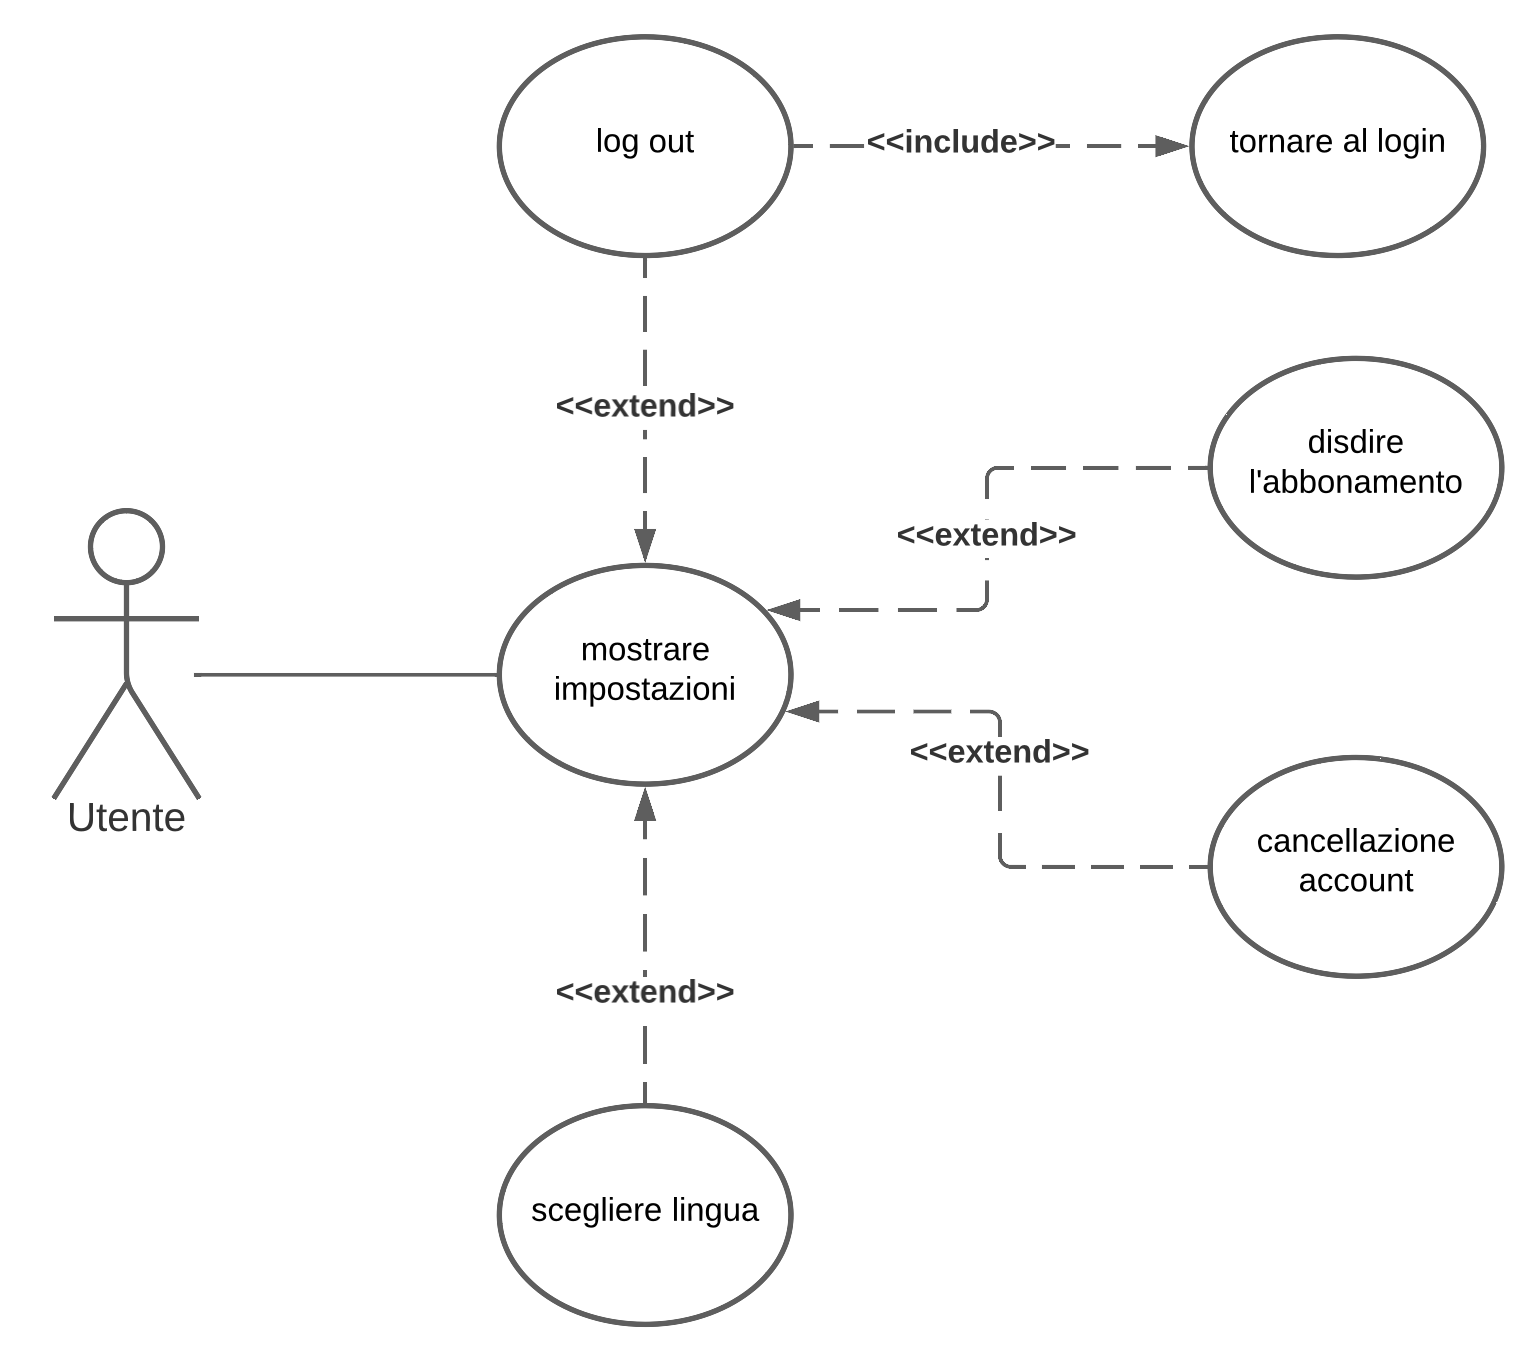
\includegraphics[width=0.75\textwidth]{diagrams/use-case-14-15-16-17-18.png}
\end{figure}

\subsubsection*{RF 14 Impostazioni}

\textbf{Descrizione:} l’utente può accedere alla pagina delle impostazioni, dalla quale può compiere una serie di azioni relative al proprio account e alla piattaforma.

\subsubsection*{RF 15 Logout}

\textbf{Descrizione:} l’utente può disconnettersi dalla piattaforma. \newline
\textbf{Passi:}
\begin{enumerate}
    \item L’utente si reca alla pagina delle impostazioni
    \item L’utente preme un pulsante per effettuare la disconnessione del proprio account
    \item L’utente viene riportato alla pagina di login
\end{enumerate}

\subsubsection*{RF 16 Cancellazione account}

\textbf{Descrizione:} l’utente può richiedere la rimozione del suo account dalla piattaforma. \newline
\textbf{Passi:}
\begin{enumerate}
    \item L’utente si reca alla pagina delle impostazioni
    \item L’utente preme un pulsante per terminare richiedere l'eliminazione del suo account
    \item L’utente creator conferma la scelta
    \item L'utente viene riportato alla schermata di registrazione
\end{enumerate}

\subsubsection*{RF 17 Disdire l'abbonamento}

\textbf{Descrizione:} l’utente può disconnettersi dalla piattaforma. \newline
\textbf{Passi:}
\begin{enumerate}
    \item L’utente si reca alla pagina delle impostazioni
    \item L’utente preme un pulsante per terminare l’abbonamento alla piattaforma
    \item L’utente potrà usufruire del servizio fino al termine del mese per il quale ha pagato
    \item Una volta terminato quel periodo, dopo l’accesso alla piattaforma l’utente sarà portato alla pagina del pagamento
\end{enumerate}

\subsubsection*{RF 18 Cambio lingua}

\textbf{Descrizione:}  l’utente può cambiare la lingua della piattaforma. \newline
\textbf{Passi:}
\begin{enumerate}
    \item L'utente si reca alla pagina delle impostazioni
    \item L’utente tramite un menù a tendina può scegliere la lingua di visualizzazione della piattaforma
    \item Il servizio si adatta, modificando i vari campi testuali per riflettere la lingua selezionata dall’utente
\end{enumerate}

\subsection*{RF 19-20}

\begin{figure}[htp]
    \centering
    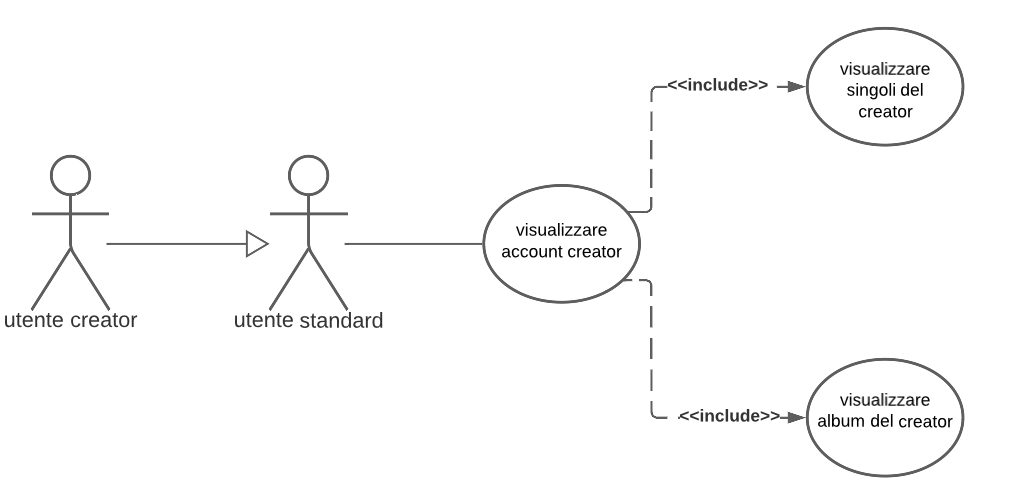
\includegraphics[width=0.75\textwidth]{diagrams/use-case-19-20.png}
\end{figure}

\subsubsection*{RF 19 Account creator}

\textbf{Descrizione:} l’account creator consiste in un'estensione dell'account standard.

\subsubsection*{RF 20 Visualizzare account creator}

\textbf{Descrizione:} gli utenti creator e gli utenti standard possono visualizzare le pagine degli account creator. Qui sono presenti due elenchi: i singoli caricati e gli album caricati da quel creator.

\subsection*{RF21 Caricare releases}

\begin{figure}[htp]
    \centering
    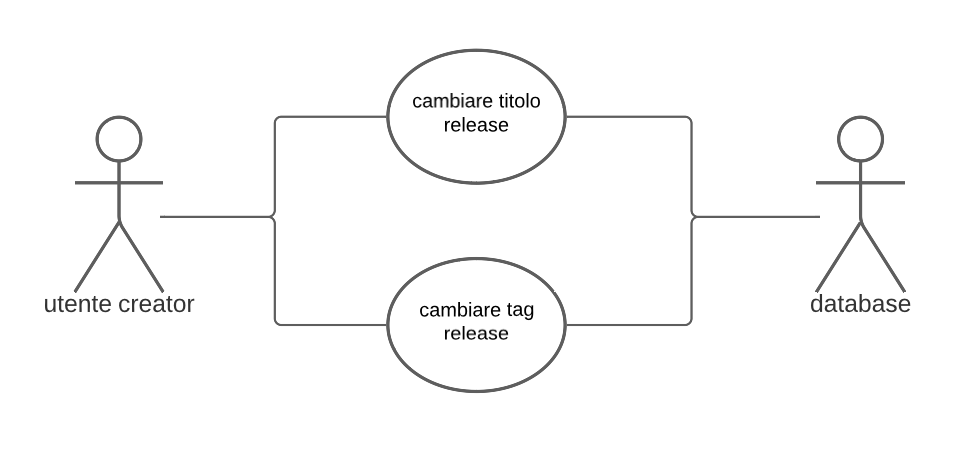
\includegraphics[width=0.75\textwidth]{diagrams/use-case-21.png}
\end{figure}

\textbf{Descrizione:} questo use case descrive il caricamento delle releases sulla piattaforma da parte dei creator.

\textbf{Passi:}
\begin{enumerate}
    \item L’utente creator sceglie di caricare una release dalla sua pagina
    \item L’utente creator seleziona la release da caricare tramite il browser
    \item L’utente creator sceglie il titolo da assegnare alla release \textbf{[extension 1]}
    \item L’utente creator conferma la scelta
    \item La release viene salvata sul database della piattaforma
\end{enumerate}
\textbf{[extension 1]} L’utente creator può aggiungere dei tag alla release caricata.

\subsection*{RF22 Modificare releases}

\begin{figure}[htp]
    \centering
    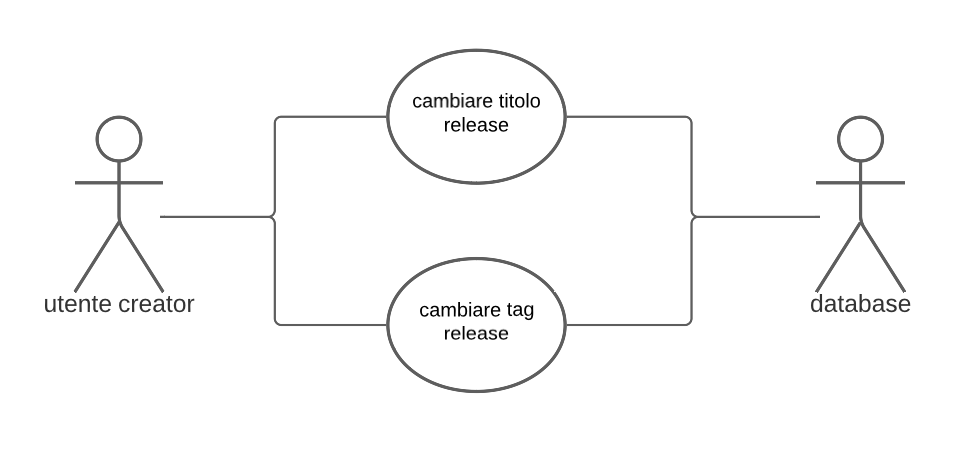
\includegraphics[width=0.75\textwidth]{diagrams/use-case-22.png}
\end{figure}

\textbf{Descrizione:} gli utenti creator possono modificare il titolo e i tag delle releases che hanno caricato sulla piattaforma. Questo dalla schermata del loro account.

\textbf{Passi:}
\begin{enumerate}
    \item L’utente creator seleziona una release dalla propria pagina
    \item L'utente sceglie l’opzione di modifica
    \item L'utente può da qui modificare il titolo, i tag, o entrambi
    \item Le modifiche vengono salvate nel database
    
\end{enumerate}

\subsection*{RF23 Eliminare releases}

\begin{figure}[htp]
    \centering
    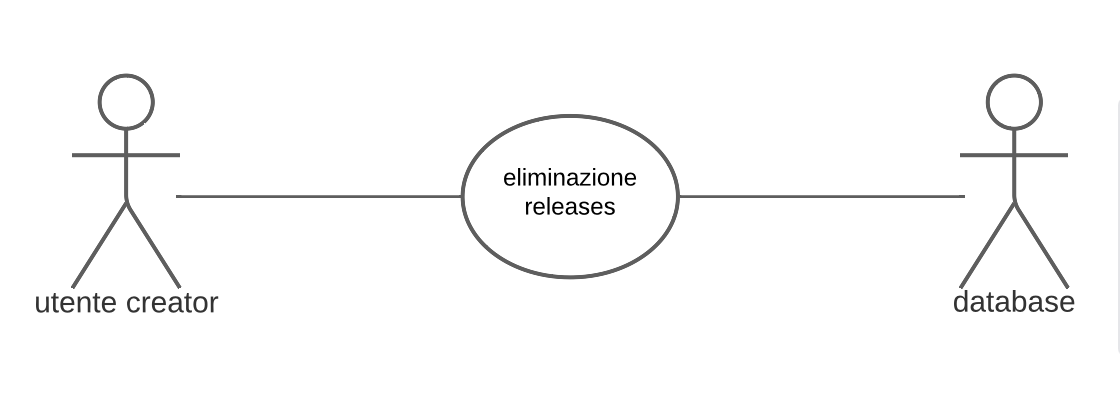
\includegraphics[width=0.75\textwidth]{diagrams/use-case-23.png}
\end{figure}

\textbf{Descrizione:} gli utenti creator possono cancellare dalla piattaforma releases da loro caricate. Questo dalla schermata del loro account.

\textbf{Passi:}
\begin{enumerate}
    \item L’utente creator seleziona una release dalla propria pagina
    \item L'utente sceglie l’opzione di eliminazione
    \item L'utente conferma l’eliminazione della release dalla piattaforma
    \item La release viene rimossa dal database    
\end{enumerate}

\newpage
\section{Requisiti non funzionali}

Presentiamo i requisiti non funzionali del progetto. Ciascun requisito è accompagnato da una misura che, quando raggiunta, trasmette se il corrispondente requisito è stato raggiunto.

\subsection*{Portabilità}

{
    \centering
    \begin{tabularx}{\textwidth}{|l|>{\raggedright\arraybackslash}X|>{\raggedright\arraybackslash}X|>{\raggedright\arraybackslash}X|}
    \hline
    Portabilità & Il servizio deve essere accessibile dai browser di computer fissi e portatili. Deve supportare i principali browser in commercio. & Le versioni dei browser Safari, Edge, Firefox, Chrome, rilasciate entro il 2017 devono supportare le funzionalità del software. \\
    \hline
    \end{tabularx} \par
}
\subsection*{Security}
{
    \centering
    \begin{tabularx}{\textwidth}{|l|>{\raggedright\arraybackslash}X|>{\raggedright\arraybackslash}X|>{\raggedright\arraybackslash}X|}
    \hline
    Password sicura & Gli utenti possono associare al proprio account solamente una password sicura. & Per essere classificata come sicura, la password deve avere una lunghezza minima di 8 caratteri, una lettera maiuscola, una lettera minuscola, un carattere speciale (\%\&\#!@*\textasciicircum). \\
    \hline
    Email verificata & L’indirizzo email inserito dall’utente deve essere verificato come esistente e in suo possesso. & Quando l’utente clicca il pulsante per la registrazione, una mail viene inviata all’indirizzo inserito dall’utente contenente un link da cliccare. Una volta cliccato il link, la mail viene validata. \\
    \hline
    Protezione della trasmissione & La trasmissione dati tra il browser dell’utente e il server web del sistema deve essere cifrata. & Deve essere usato il protocollo https. \\
    \hline
    Protezione diritti d'autore & Il software deve fare il possibile per prevenire la diffusione non autorizzata delle releases disponibili. & \\
    \hline
    \end{tabularx} \par
}
\subsection*{Recupero password}

{
    \centering
    \begin{tabularx}{\textwidth}{|l|>{\raggedright\arraybackslash}X|>{\raggedright\arraybackslash}X|>{\raggedright\arraybackslash}X|}
    \hline
    Recupero password & L’utente deve essere in grado di accedere al suo account anche nel caso in cui abbia dimenticato la password. & Nella pagina di registrazione è disponibile un bottone per recuperare la password attraverso l’indirizzo email associato all’account. \\
    \hline
    \end{tabularx} \par
}
\subsection*{Cambiare la password}

{
    \centering
    \begin{tabularx}{\textwidth}{|l|>{\raggedright\arraybackslash}X|>{\raggedright\arraybackslash}X|>{\raggedright\arraybackslash}X|}
    \hline
    Cambiare la password & L’utente loggato deve essere in grado di cambiare la password associata al suo account. & Dalle impostazioni dev’essere possibile inserire una nuova password per sostituire quella corrente. \\
    \hline
    \end{tabularx} \par
}
\subsection*{Affidabilità}

{
    \centering
    \begin{tabularx}{\textwidth}{|l|>{\raggedright\arraybackslash}X|>{\raggedright\arraybackslash}X|>{\raggedright\arraybackslash}X|}
    \hline
    Ridondanza & L’infrastruttura è ridondata per garantire la protezione dal fallimento dei dischi. & Devono essere presenti almeno due istanze del servizio, per cui la terminazione di una non intacchi la disponibilità del servizio. La perdita di servizio dev’essere automaticamente segnalata all’amministratore. \\ \hline
    Backup & Devono essere presenti dei backup del sito in modo da recuperare i dati in caso di guasti o attacchi hacker. & I backup devono comprendere tutti i dati del sistema. Sono eseguiti mensilmente. Sono salvati su un servizio esterno. \\
    \hline
    \end{tabularx} \par
}
\subsection*{Usabilità}

{
    \centering
    \begin{tabularx}{\textwidth}{|l|>{\raggedright\arraybackslash}X|>{\raggedright\arraybackslash}X|>{\raggedright\arraybackslash}X|}
    \hline
    Familiarità & L’applicazione deve risultare familiare e facile da utilizzare. & Giovani adulti di età compresa tra i 16 e i 35 anni, previa esperienza di un recente dispositivo digitale (dal 2015 in poi) devono riuscire ad usufruire del servizio senza necessitare di aiuto esterno (almeno 50 utenti di test). \\
    \hline
    \end{tabularx} \par
}
\subsection*{Privacy}

{
    \centering
    \begin{tabularx}{\textwidth}{|l|>{\raggedright\arraybackslash}X|>{\raggedright\arraybackslash}X|>{\raggedright\arraybackslash}X|}
    \hline
    GDPR & Conforme al regolamento generale sulla protezione dei dati in sigla GDPR, ufficialmente regolamento n. 2016/679. & Il software permette la cancellazione dei dati personali che lo riguardano senza ingiustificato ritardo. Permette inoltre all’utente di ottenere la conferma che sia o meno in corso un trattamento di dati personali che lo riguardano. \\
    \hline
    \end{tabularx} \par
}
\subsection*{Performance}

{
    \centering
    \begin{tabularx}{\textwidth}{|l|>{\raggedright\arraybackslash}X|>{\raggedright\arraybackslash}X|>{\raggedright\arraybackslash}X|}
    \hline
    Qualità dell'audio & Lo streaming deve adattarsi alla banda disponibile all’utente. & Il servizio deve garantire lo streaming ad un minimo 160 kbps di banda e fino ad un massimo di 320 kbps. \\ \hline
    Velocità di ricerca & La ricerca all’interno del sistema deve avvenire in un tempo accettabile. & I risultati dalla barra di ricerca vengono restituiti entro 10 secondi, con una media di 3 secondi. \\
    \hline
    \end{tabularx} \par
}
\subsection*{Pagamento}

{
    \centering
    \begin{tabularx}{\textwidth}{|l|>{\raggedright\arraybackslash}X|>{\raggedright\arraybackslash}X|>{\raggedright\arraybackslash}X|}
    \hline
    Pagamento & Si usufruisce al servizio sulla base di un pagamento ricorrente. & Il pagamento avviene mensilmente; il giorno corrisponde al giorno della sottoscrizione al servizio da parte dell’utente. La piattaforma sfrutta il servizio di pagamento scelto dall’utente per prelevare la quota necessaria. \\
    \hline
    \end{tabularx} \par
}
\subsection*{Tag}

{
    \centering
    \begin{tabularx}{\textwidth}{|l|>{\raggedright\arraybackslash}X|>{\raggedright\arraybackslash}X|>{\raggedright\arraybackslash}X|}
    \hline
    Tag & Ogni release possiede dei tag che la caratterizzano. & Ciascuna release deve essere associata ad un minimo di 3 (tre) tag. \\
    \hline
    \end{tabularx} \par
}

\newpage
\section{Diagramma di contesto}

Presentiamo ora un'analisi del contesto nel quale si inserirà il nostro progetto. Per fare ciò, terremo in considerazione i sistemi e gli attori con i quali la nostra piattaforma andrà ad interagire e gli attori. L'analisi sarà costituita da una descrizione testuale di attori e sistemi e da un diagramma di contesto che riassume la situazione.

\subsection{Attori e sistemi esterni}

\paragraph{Utente} La persona che si registrerà e pagherà per il servizio, che comprende la riproduzione di brani in streaming e la gestione di playlist definite dall’utente. Oltre questo, l’utente riceve consigli dal sistema e può dare del feedback a riguardo. L’utente deve inoltre essere capace di cambiare qualche impostazione, tra cui gestire l’abbonamento.

\paragraph{Creator} L’utente creator, oltre a poter fruire del servizio come ogni normale utente, è anche capace di pubblicare i propri brani come releases.

\paragraph{Sistema Pagamento} Attraverso il sistema di pagamento il sistema manda con cadenza mensile i pagamenti attraverso il metodo utilizzato dall’utente.

\paragraph{Mail Server} Attraverso il mail server il sistema manda emails (ad esempio per verificare l’email inserita in fase di registrazione, per il cambio della password in caso di smarrimento, etc.).

\paragraph{Database} Il database tiene separatamente le informazioni riguardo utenti e releases.

\paragraph{DRM} Il Digital Rights Management system si preoccupa di proteggere i files per rendere difficile la pirateria

\paragraph{CDN}: La rete che si preoccupa di diffondere il brano in diversi punti di internet in modo da servire più velocemente diversi utenti dispersi nel mondo.

\paragraph{Backup}: I server che si preoccupano di hostare i backups dei server principali, in modo da mantenere un archivio storico e sostenere attacchi informatici o sopportare eventuali problemi hardware.

\paragraph{Diagnosi}: I server che ricevono periodicamente i logs del sistema, per una più facile analisi di eventuali problematiche e profilazione delle performance.

\newpage
\subsection{Diagramma di contesto}

\begin{figure}[htp]
    \centering
    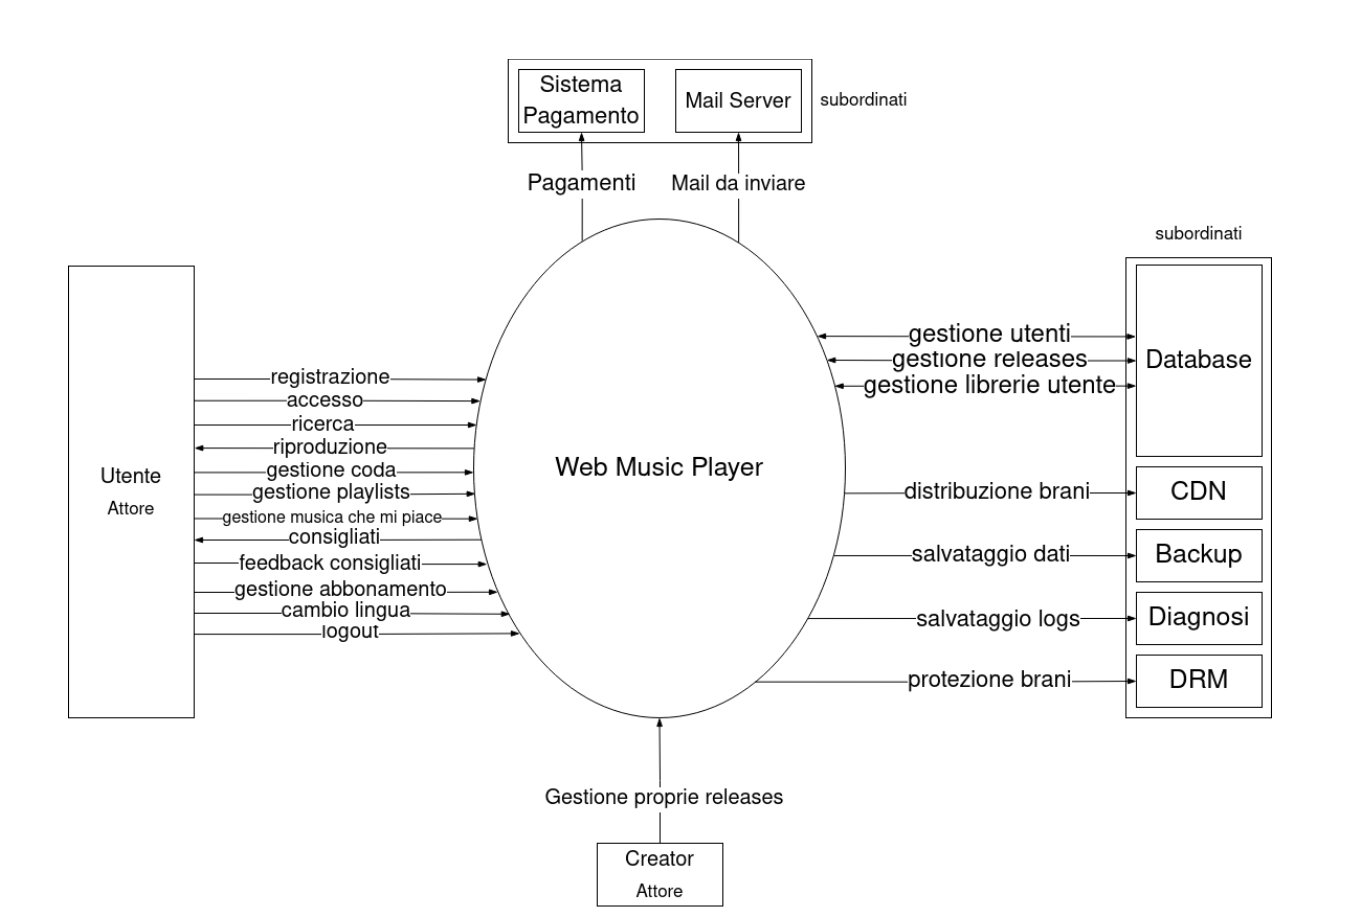
\includegraphics[width=\textwidth]{diagrams/context.png}
\end{figure}

\newpage
\section{Diagramma delle componenti}

Dopo il contesto nel quale si inserirà il nostro sistema, andiamo ad analizzare le varie componenti che lo formano. L'analisi sarà formata da una descrizione testuale di ciascuna componente e delle sue interfacce in entrata e in uscita. Terminerà con un diagramma delle componenti.

\subsection{Analisi delle componenti}

\subsubsection{Registrazione}

\underline{Descrizione}: questa componente si occupa di interfacciarsi con l’utente durante la fase di registrazione, come da RF1. I dati per la registrazione verranno prelevati e inviati ad altre componenti.

\underline{Interfaccia richiesta - Email e password}: questa componente richiede l'inserimento di indirizzo email e password da parte dell'utente. In particolare, la password andrà inserita due volte. All'inserimento di queste viene effettuato un rapido controllo della sintassi, per far sì che l'email possa corrispondere ad un indirizzo valido e che la password rispetti i requisiti di sicurezza (RNF2a).

\underline{Interfaccia richiesta - Tipo di account}: l’utente seleziona la tipologia dell’account che intende creare. Le scelte disponibili sono Utente standard e Utente creator.

\underline{Interfaccia richiesta - Conferma email}: per completare la registrazione è necessario ricevere una conferma della validitaà dell'indirizzo email. Questa informazione si ha nella forma di una conferma inviata da un'altra componente, la quale indica che l’utente in questione eè in proprietario dell'indirizzo email inserito.

\underline{Interfaccia richiesta - Token utente}: viene richiesto l’identificativo per l’utente appena registrato. Una volta completata la registrazione, questo identificativo viene inviato ad un’altra componente.

\underline{Interfacce fornita - Token utente}: una volta terminata la registrazione, questa componente fornisce l’identificativo all’interno della piattaforma dell’utente appena inserito.

\underline{Interfaccia fornita - Email utente}: per la registrazione è necessario che l’indirizzo email dell’utente sia validato. Questa interfaccia fornisce l’indirizzo email ad una componente che si occupa di questa validazione.

\underline{Interfaccia fornita - Dati registrazione}: questa interfaccia fornisce le informazioni raccolte durante la registrazione. Queste includono indirizzo email, password e tipo di account scelto dall’utente.

\subsubsection{Pagamento}

\underline{Descrizione}: questa componente si occupa della gestione delle operazioni relative al pagamento della quota mensile per la piattaforma, come da RF2. Una volta ricevuti i dati dell’utente, si occuperà della scelta del servizio di pagamento e dell’effettuare il pagamento ricorrente. Quest’ultimo può essere interrotto.

\underline{Interfaccia richiesta - Token utente}: la componente necessità dell’identificativo dell’utente per associare le operazioni di pagamento all’account specifico presente sulla piattaforma. 

\underline{Interfaccia richiesta - Conferma pagamento}: viene richiesta al servizio di pagamento contattato una conferma dell’avvenuto pagamento.

\underline{Interfaccia fornita - Richiesta pagamento}: una volta che l’utente avrà selezionato il metodo di pagamento utilizzare, questa interfaccia si occupa di contattare il servizio scelto con un identificativo dell’utente.

\subsubsection{Validazione mail}

\underline{Descrizione}: questa componente si occupa dell’interazione con il servizio esterno per le email con cui interagisce nostro sistema, come da RNF2b. Il servizio viene utilizzato per verificare che un utente che interagisce col sistema sia in possesso dell’indirizzo email che sceglie di inserire.

\underline{Interfaccia richiesta - Email utente}: la componente richiede un indirizzo email al quale dovrà essere inviata la email di conferma.

\underline{Interfaccia richiesta - Conferma email}: il servizio esterno comunica alla componente se l’utente ha cliccato il link presente nell’email inviata all’indirizzo email specificato. Questa comunicazione consiste nella conferma dell’indirizzo.

\underline{Interfaccia fornita - Email utente}: la componente fornisce al servizio esterno per l’invio delle email l’indirizzo ricevuto da altre componenti, al quale dovrà essere inviata la email.

\underline{Interfaccia fornita - Conferma email}: questa interfaccia fornisce ad altre componenti la conferma dell’indirizzo email ricevuto, ovvero se l’indirizzo email inserito dall’utente gli appartiene.

\subsubsection{Recupero password}

\underline{Descrizione}: questa componente si occupa del recupero della password da parte dell’utente, come da RF4, RNF3. Viene anche usata per il cambio della password all’interno della piattaforma, come da RNF4. In entrambi i casi, viene utilizzato l’indirizzo email associato all’account per verificare l’identità dell’utente in questione. Una volta fatto ciò, viene data la possibilità di impostare una nuova password per l’account.

\underline{Interfaccia richiesta - Email utente}: per avviare il processo di recupero password è necessario l’indirizzo email associato all’account.

\underline{Interfaccia richiesta - Conferma esistenza email}: viene richiesta una conferma dell’esistenza di un account con associato l’indirizzo email inserito dall’utente. Questa conferma è necessaria per continuare il processo di recupero.

\underline{Interfaccia richiesta - Conferma email}: è necessario ricevere la conferma del fatto che l’utente che abbia inserito l’indirizzo ne sia effettivamente in possesso. Questa conferma è ricevuta da un’altra componente.

\underline{Interfaccia fornita - Email utente}: dopo l’inserimento dell’email da parte dell’utente, è necessario verificare che si tratti di un indirizzo effettivamente associato ad un account. Questa verifica è compiuta da un’altra componente, alla quale viene fornito l’indirizzo da questa interfaccia.

\underline{Interfaccia fornita - Nuova password}: una volta terminate le verifiche sull’indirizzo email, viene inserita una nuova password da parte dell’utente, la quale dovrà essere salvata nella piattaforma. Questa operazione di salvataggio è compiuta dalla componente alla quale quest’interfaccia comunica la nuova password.

\subsubsection{Login}

\underline{Descrizione}: questa componente si occupa di gestire l’accesso di un utente registrato alla piattaforma, come da RF3.

\underline{Interfaccia richiesta - Email e password}: l’utente anonimo inserisce le proprie credenziali, email e password.

\underline{Interfaccia richiesta - Token utente}: per procedere con l’accesso è necessaria una conferma dell’esistenza dell’utente all’interno della piattaforma. Se questa conferma non viene ricevuta, l’accesso viene negato.

\underline{Interfaccia richiesta - Stato pagamenti}: una volta confermata l’esistenza dell’utente nel sistema, viene richiesto lo stato dei suoi pagamenti. Se l’utente registrato deve ancora procedere nel pagamento del mese in questione, viene ricondotto alla pagina per il pagamento.

\underline{Interfaccia fornita - Credenziali}: le credenziali inserite dall’utente vengono fornite ad \\ un’altra componente. Questa dovrà verificare l’esistenza dell’utente sulla piattaforma.

\underline{Interfaccia fornita - Token utente}: una volta verificato che l’utente che ha inserito le credenziali sia registrato nel sistema, questa interfaccia fornisce l’identificativo dell’utente ad altre componenti che lo necessitano.

\subsubsection{Impostazioni}

\underline{Descrizione}: questa componente consente all’utente di effettuare le seguenti operazioni: effettuare il logout (RF15), disdire l’abbonamento (RF16), cambiare la lingua di visualizzazione (RF17), cambiare la password associata all’account (RNF4), richiedere la cancellazione dell'account. Effettuare il logout rimanda alla pagina di login, non è richiesto alcuno scambio di informazioni. Componenti diverse si occupano delle altre funzioni.

\underline{Interfaccia richiesta - Operazione da eseguire}: questa componente richiede all’utente di scegliere quale operazione eseguire tra quelle disponibili.

\underline{Interfaccia richiesta - Token utente}: viene richiesto l’identificativo dell’utente dopo l’accesso alla piattaforma, per legare all’account corretto le varie operazioni che si possono effettuare.

\underline{Interfaccia fornita - Token utente}: nel caso in cui l’operazione scelta richieda un’azione da parte di un’altra componente, è necessario comunicare a quest’ultima l’identificativo dell’utente.

\underline{Interfaccia fornita - Email utente}: nel caso in cui l’operazione scelta sia il cambio password, viene fornita l’email dell’utente che intende svolgere l’operazione ad una componente apposita.

\underline{Interfaccia fornita - Lingua scelta}: nel caso in cui l’operazione scelta sia il cambio della lingua di visualizzazione, questa modifica viene comunicata ad un’altra componente che la implementerà.

\subsubsection{Anagrafica database}

\underline{Descrizione}: questa componente si occupa dell’interazione con il database esterno al sistema per quanto riguarda i dati relativi agli account degli utenti.

\underline{Interfaccia richiesta - Dati registrazione}: questa interfaccia riceve i dati di un nuovo utente che intende completare la registrazione e li inserisce nel database esterno utilizzato dal sistema.

\underline{Interfaccia richiesta - Credenziali}: questa interfaccia riceve le credenziali, quindi email e password, di un utente e verifica due cose: la loro presenza nel database e la corretta associazione tra le due.

\underline{Interfaccia richiesta - Email utente}: questa interfaccia riceve un’email inserita da un utente e verifica la sua presenza nel database.

\underline{Interfaccia richiesta - Nuova password}: questa interfaccia richiede una password da associare ad un indirizzo email all’interno del database.

\underline{Interfaccia richiesta - Dati utente nel DB}: questa interfaccia richiede i dati di un utente all’interno del database. Per fare ciò, fornisce le credenziali ad esso associate.

\underline{Interfaccia richiesta - Lingua scelta}: questa interfaccia riceve una modifica sulla lingua di visualizzazione preferita da un utente e la salva nel database.

\underline{Interfaccia fornita - Token utente}: questa interfaccia riceve l’identificativo di un utente già presente nella piattaforma.

\underline{Interfaccia fornita - Dati utente da inserire}: questa interfaccia fornisce al database esterno i dati da inserire per la registrazione di un nuovo utente.

\underline{Interfaccia fornita - Token utente}: questa interfaccia fornisce l’identificativo di un utente recuperato dal database esterno. Per il recupero sono state utilizzate le credenziali associate a quell’utente.

\underline{Interfaccia fornita - Conferma email}: questa interfaccia fornisce una conferma dell’esistenza di un’email all’interno del database.

\underline{Interfaccia fornita - Stato pagamenti}: questa interfaccia fornisce lo stato attuale dei pagamenti di un utente. In particolare, se il giorno corrente rientra in un periodo coperto dall’ultimo pagamento registrato per un certo account.

\subsubsection{Caricamento dati utente}

\underline{Descrizione}: questa componente si occupa del prelievo dal database di tutti i dati di un particolare utente necessari quando quest’ultimo si logga. Questa componente si occupa di dividere questi dati e inviarli alle componenti corrispondenti.

\underline{Interfaccia richiesta - Token utente}: viene richiesto un token per identificare l’utente che si è appena loggato.  La componente preleva questo dato e lo utilizza per prelevare informazioni nel database.

\underline{Interfaccia richiesta - Dati utente}: vengono richiesti i dati utente dal database. La componente Gestione prelievo dati spartirà e invierà questi dati alle corrispondenti componenti.

\underline{Interfaccia fornita - Token utente}: Il token utente viene fornito alla componente Database.

\underline{Interfaccia fornita - Dati cronologia}: questa interfaccia fornisce ad un altro componente tutti i dati riguardanti la cronologia di un particolare utente.

\underline{Interfaccia fornita - Dati consigliati}: questa interfaccia fornisce alla componente successiva tutti i dati riguardanti i brani che il sistema consigliava all’utente nel precedente login.  

\underline{Interfaccia fornita - Dati libreria}: questa interfaccia fornisce tutti i dati e le informazioni utili alla gestione della libreria di un particolare utente, in particolare vengono scambiate tutte le informazioni riguardanti i brani che piacciono all’utente e tutte le sue playlist salvate.

\subsubsection{Libreria}

\underline{Descrizione}: questa componente si occupa di gestire tutti i dati riguardanti la libreria; questi comprendono i brani che piacciono all’utente e le playlist salvate. Deve inoltre gestire tutte le azioni che possono essere effettuate sulla libreria tra cui l’aggiunta, eliminazione, riproduzione di brani e playlist.

\underline{Interfaccia richiesta - Dati libreria}: Questa interfaccia richiede i dati riguardanti la libreria.

\underline{Interfaccia richiesta - Azioni libreria}: Questa interfaccia prende in ingresso tutte le azioni che l’utente può svolgere sulla libreria. Le azioni possono essere ad esempio: aggiunta di brani ad una playlist, eliminazione di brani, rinomina di una playlist e in particolare di una playlist per la visualizzazione e il successivo ascolto dei brani salvati al suo interno.

\underline{Interfaccia richiesta - Selezione release}: questa interfaccia prende in ingresso la selezione di una release che l’utente vuole ascoltare.

\underline{Interfaccia fornita - Token raccolta}: questa interfaccia serve a fornire alla componente successiva il Token raccolta, che verrà utilizzato per la gestione di un interfaccia che mostra i brani della playlist selezionata dall’utente.

\underline{Interfaccia fornita - Info brani in libreria}: questa interfaccia fornisce tutte le informazioni utili alla componente successiva (Gestione scelte canzoni suggerite) per la selezione di nuovi brani da consigliare. Queste informazioni sono: nome artista, tag brano, lunghezza brano.

\underline{Interfaccia fornita - Token release}: questa interfaccia fornisce il Token (identificativo) di una determinata release alla componente successiva.

\underline{Interfaccia fornita - Libreria aggiornata}: questa interfaccia fornisce ad un'altra componente i dati aggiornati della libreria per fare in modo che questi possano essere salvati sul database.

\subsubsection{Gestione releases creator}

\underline{Descrizione}: questa componente si occupa della gestione di tutti i dati appartenenti all’account creator e di tutte le operazioni che quest’ultimo può fare.

\underline{Interfaccia richiesta - release}: questa interfaccia richiede l’input da parte dell’utente creator di una determinata release che può essere un brano o un album. 

\underline{Interfaccia richiesta - Modifiche (Titolo/tag)}: questa interfaccia prende in ingresso tutte le modifiche che l’utente creator può effettuare. Le modifiche possono essere: titolo, tag.

\underline{Interfaccia richiesta - Eliminazione}: questa interfaccia permette l’eliminazione di una propria release da parte dell’utente creator.

\underline{Interfaccia fornita - Azioni release}: questa interfaccia fornisce alla componente successiva (Gestione Database) tutte le aggiunte e modifiche da applicare al database in seguito alle azioni compiute dall’utente creator.

\subsubsection{Cronologia}

\underline{Descrizione}: questa componente si occupa della cronologia di visualizzazione di un utente, come da RF13. Mostra gli ultimi 30 brani ascoltati dall’utente in ordine cronologico inverso.

\underline{Interfaccia richiesta - Dati cronologia}: questa interfaccia riceve i dati relativi alla cronologia di un determinato utente

\underline{Interfaccia richiesta - Token brano riprodotto}: questa interfaccia riceve l’identificativo di un brano quando viene messo in riproduzione, così da poterlo aggiungere alla cronologia.

\underline{Interfaccia fornita - Token brano}: questa interfaccia fornisce l’identificativo di un brano ad un’altra componente nel momento in cui il brano viene selezionato per la riproduzione da parte dell’utente.

\underline{Interfaccia fornita - Info ascolti passati}: questa interfaccia fornisce ad un’altra componente le informazioni relative agli ascolti passati dell’utente.

\underline{Interfaccia fornita - Cronologia aggiornata}: la cronologia viene aggiornata dall’ascolto di nuovi brani. Viene man mano inviata ad un’altra componente che si occuperà del salvataggio di questi cambiamenti.

\subsubsection{Consigliati}

\underline{Descrizione}: questa componente si occupa dell’elenco dei brani consigliati all’utente da parte della piattaforma, come da RF11. Raggruppa i brani consigliati all’utente e i controlli di feedback per ciascun brano.

\underline{Interfaccia richiesta - Dati consigliati}: questa interfaccia riceve i dati relativi ai brani consigliati ad un determinato utente.

\underline{Interfaccia richiesta - Feedback}: questa interfaccia riceve il feedback relativo ad uno specifico brano consigliato da parte dell’utente. Il feedback viene dato tramite appositi controlli sul lato di ogni brano.

\underline{Interfaccia richiesta - Brani scelti per l’utente}: questa interfaccia riceve gli identificativi e alcune informazioni sui brani che un’altra componente ha scelto come suggerimenti. I dati ricevuti includono il titolo del brano e l’artista, così da poterli mostrare all’utente, e l’identificativo, da poter inviare ad altre componenti.

\underline{Interfaccia fornita - Token brano}: questa interfaccia fornisce l’identificativo di un brano ad un’altra componente nel momento in cui il brano viene selezionato per la riproduzione da parte dell’utente.

\underline{Interfaccia fornita - Dati ascolti passati}: questa interfaccia fornisce ad un’altra componente le informazioni relative ai brani consigliati all’utente in passato.

\underline{Interfaccia fornita - Feedback utente}: il feedback ricevuto dall’utente relativo a dei brani consigliati viene consegnato ad un’altra componente.

\subsubsection{Scelta canzoni suggerite}

\underline{Descrizione}: questa componente si occupa della scelta dei brani da suggerire all’utente; racchiude quindi l’algoritmo che si occupa dei suggerimenti. Per produrre dei buoni suggerimenti, lavora con i dati ricevuti dalla libreria, con i dati sugli ascolti passati, sui brani consigliati in passato e con il feedback dell’utente su quei brani.

\underline{Interfaccia richiesta - Info brani in libreria}: questa interfaccia riceve dati relativi alle releases e alle playlists presenti nella libreria di un determinato utente.

\underline{Interfaccia richiesta - Info ascolti passati}: questa interfaccia riceve la cronologia di ascolto di un determinato utente.

\underline{Interfaccia richiesta - Dati consigliati passati}: questa interfaccia riceve informazioni relative ai brani che sono stati consigliati ad un determinato utente.

\underline{Interfaccia richiesta - Dati brani}: questa interfaccia richiede dei dati relativi ad alcuni brani. Questi includono brani di artisti ascoltati dall’utente, con dei tag che si avvicinano a quelli dei brani che l’utente ascolta di frequente, etc.

\underline{Interfaccia richiesta - Feedback utente}: questa interfaccia richiede le informazioni sul \\ feedback che l’utente ha dato rispetto ai brani che gli sono stati suggeriti.

\underline{Interfaccia fornita - Token brani}: questa interfaccia fornisce gli identificativi dei brani che la componente ha richiesto.

\underline{Interfaccia fornita - Brani scelti per l’utente}: questa interfaccia invia ad un’altra componente i brani che potrebbero piacere all’utente, sulla base dei dati analizzati.

\subsubsection{Ricerca}

\underline{Descrizione}: questa componente si occupa di gestire la ricerca di releases, artisti o playlists all’interno della piattaforma, come da RF5.

\underline{Interfaccia richiesta - Testo della ricerca}: questa interfaccia riceve in input il testo della ricerca dell’utente, ciò che deve essere cercato all’interno della piattaforma.

\underline{Interfaccia richiesta - Risultato ricerca}: questa interfaccia riceve il risultato della ricerca all’interno del database della piattaforma. Questo consiste in un elenco dei vari identificativi

\underline{Interfaccia fornita - Testo della ricerca}: questa interfaccia fornisce ad un’altra componente il testo della ricerca dell’utente.

\underline{Interfaccia fornita - Token raccolta}: questa interfaccia fornisce ad un’altra componente l’identificativo della raccolta trovata nella ricerca. Questa può essere un album o una playlist dell’utente.

\underline{Interfaccia fornita - Token brano}: questa interfaccia fornisce l’identificativo di un brano trovato nella ricerca ad un’altra componente, nel momento in cui il brano viene selezionato per la riproduzione da parte dell’utente.

\underline{Interfaccia fornita - Token artista}: questa interfaccia fornisce ad un’altra componente l’identificativo di un artista trovato nella ricerca.

\subsubsection{Raccolte}

\underline{Descrizione}: questa componente si occupa del raggruppamento e modifica di raccolte musicali, ovvero di album e playlists. Per una raccolta presenta il titolo, l’elenco dei brani ed eventuali opzioni di modifica. Le modifiche sono concesse nel caso in cui la raccolta in questione sia una playlist.

\underline{Interfaccia richiesta - Token raccolta}: per visualizzare una raccolta è necessario il suo identificativo all’interno della piattaforma; questa è l’interfaccia che lo riceve.

\underline{Interfaccia richiesta - Dati raccolta}: questa interfaccia si occupa del ricevere i dati relativi ad una raccolta da un’altra componente.

\underline{Interfaccia richiesta - Brano selezionato}: questa interfaccia riceve un eventuale richiesta di riproduzione di un brano da parte dell’utente.

\underline{Interfaccia richiesta - Azioni raccolta}: questa interfaccia riceve dall’utente eventuali azioni relative alla raccolta corrente. Queste includono l’aggiunta o eliminazione di nuovi brani, o il cambiamento del titolo della raccolta.

\underline{Interfaccia fornita - Token brano}: questa interfaccia fornisce l’identificativo del brano da riprodurre ad un’altra componente.

\underline{Interfaccia fornita - Token raccolta}: questa interfaccia si occupa di fornire l’identificativo di una raccolta ad un’altra componente, per il recupero dei dati relativi a quella raccolta.

\underline{Interfaccia fornita - Azioni raccolta}: questa interfaccia si occupa di trasmettere i cambiamenti avvenuti ad una raccolta per via di azioni compiute dall’utente.

\subsubsection{Coda}

\underline{Descrizione}: questa componente si occupa della coda di riproduzione, come da RF7. Quando un brano viene riprodotto, vengono messe in coda eventuali canzoni ad essa legate, ovvero le canzoni successive nel caso in cui la canzone faccia parte di una playlist o di una release, fino alla fine. È possibile passare alla canzone successiva oppure riprodurre la coda in ordine casuale.

\underline{Interfaccia richiesta - Token brano}: identificativo del brano appena riprodotto.

\underline{Interfaccia richiesta - Fine brano}: viene fornito a questa componente il momento nel cui termina la riproduzione del brano attuale.

\underline{Interfaccia fornita - Token brano}: identificativo del brano appena riprodotto, inviato per ricevere eventuali altri brani appartenenti alla stessa raccolta.

\underline{Interfaccia fornita - Token release in coda}: la componente fornisce ad un’altra componente l’identificativo del prossimo brano in coda.

\underline{Interfaccia richiesta - Token brani nella raccolta}: questa interfaccia riceve gli identificativi dei brani legati a quello messo in riproduzione e che andranno aggiunti alla coda.

\subsubsection{Interfaccia creator}

\underline{Descrizione}: questa interfaccia presenta le informazioni relative ad un artista, come da RF19. Queste includono il nome del creator, i brani e gli album pubblicati.

\underline{Interfaccia richiesta - Brano selezionato}: questa interfaccia riceve in input il brano selezionato dall’utente dalla lista dei brani pubblicati dall’artista.

\underline{Interfaccia richiesta - Album selezionato}: questa interfaccia riceve in input l’album selezionato dall’utente dalla lista degli album pubblicati dall’artista.

\underline{Interfaccia richiesta - Dati artista}: questa interfaccia riceve i dati relativi ad un artista da un’altra componente, così da poterli mostrare.

\underline{Interfaccia richiesta - Token artista}: questa interfaccia riceve l’identificativo dell’artista i cui dati andranno mostrati. 

\underline{Interfaccia fornita - Token raccolta}: questa interfaccia  fornisce l’identificativo dell'album selezionato da parte dell’utente ad un’altra componente, che si occuperà di gestire l’interazione con la raccolta.

\underline{Interfaccia fornita - Token artista}: questa interfaccia  fornisce l’identificativo di un creator per poter poi recuperare tutti i dati relativi ad esso.

\underline{Interfaccia fornita - Token brano}: questa interfaccia fornisce l’identificativo di un brano ad un’altra componente nel momento in cui il brano viene selezionato per la riproduzione da parte dell’utente.

\subsubsection{Riproduzione}

\underline{Descrizione}: questa componente si occupa della gestione della riproduzione di un brano, come da RF6. Permette l’avvio, interruzione e ripresa della riproduzione di una canzone.

\underline{Interfaccia richiesta - Token brano}: questa interfaccia si occupa di recuperare l’identificativo del brano da riprodurre. Un brano può venir riprodotto da più punti all’interno della piattaforma, questa è l’informazione che permette alla componente di avviare la riproduzione.

\underline{Interfaccia richiesta - Dati brano da riprodurre}: questa interfaccia recupera il brano da riprodurre da un’altra componente. Qui si parla dei dati effettivi che compongono il brano.

\underline{Interfaccia fornita - Fine brano}: questa interfaccia comunica ad un’altra componente il momento in cui termina la riproduzione del brano corrente.

\underline{Interfaccia fornita - Token brano}: questa componente fornisce l’identificativo del brano da riprodurre (o che è appena stato riprodotto) ad altre componenti.

\underline{Interfaccia richiesta - Token release in coda}: questa componente riceve l'identificativo \\ della prossima canzone in coda, e quindi da riprodurre.

\subsubsection{Prelievo gruppi di dati}

\underline{Descrizione}: questa componente interagisce con la base di dati del sistema. Viene utilizzata per prelevare i dati di un artista, di una raccolta, di un utente e per effettuare ricerche.

\underline{Interfaccia richiesta - Token utente}: interfaccia che richiede un identificativo per l’utente che ha fatto il login. Questa informazione viene utilizzata per prelevare tutti i dati di quel particolare utente.

\underline{Interfaccia fornita - Dati utente}: Questa interfaccia fornisce alla componente Gestione prelievo dati tutti i dati dell’utente nel momento in cui quest’ultimo si logga.

\underline{Interfaccia richiesta - Testo ricerca}: questa interfaccia richiede il testo della ricerca dalla componente Gestione ricerca. Gestione database utilizza questa informazione per cercare all’interno del database se esiste una corrispondenza.

\underline{Interfaccia fornita - Risultato ricerca}: questa interfaccia fornisce i risultati della ricerca effettuata sul database. Questo risultato sarà un identificativo per il brano/album/playlist/\\artista che l’utente ha cercato.

\underline{Interfaccia richiesta - Token raccolta}: questa interfaccia richiede l’identificativo di una particolare raccolta. Questo token verrà utilizzato per cercare e prelevare i dati relativi a quella raccolta nel database.

\underline{Interfaccia fornita - Dati raccolta}: questa interfaccia fornisce ad una componente tutti i dati relativi ad una determinata raccolta.

\underline{Interfaccia richiesta - Token artista}: questa interfaccia richiede l’identificativo dell’artista (creator) per la visualizzazione dei suoi contenuti. Questo token verrà utilizzato per prelevare dal database i dati dell’artista.

\underline{Interfaccia fornita - Dati artista}: questa interfaccia fornisce i dati relativi ad un artista alla componente Interfaccia creator.

\underline{Interfaccia richiesta - Dati utente}: Questa interfaccia richiede dal database tutti i dati relativi ad un particolare utente. Questa operazione viene svolta nel momento in cui un utente si logga ed entra nel sito.

\underline{Interfaccia richiesta - Ricerca nel DB}: Questa interfaccia comprende la ricerca di particolare artista/releases nel database e richiede la conferma della sua presenza in esso.

\underline{Interfaccia richiesta - Dati artista}: questa interfaccia richiede tutti i dati di un particolare artista. Questi dati sono poi utilizzati per la visualizzazione dell’interfaccia dell’artista.

\underline{Interfaccia richiesta - Dati raccolta}: Questa interfaccia richiede dal database i dati di una particolare raccolta.

\subsubsection{Scrittura dati}

\underline{Descrizione}: questa componente interagisce con la base di dati del sistema. Si occupa della scrittura di tutti i dati relativi all'esperienza di utilizzo della piattaforma.

\underline{Interfaccia richiesta - Cronologia aggiornata}: questa interfaccia richiede i dati aggiornati dalla componente Gestione cronologia. Questi dati vengono utilizzati per aggiornare il database.

\underline{Interfaccia richiesta - Azioni releases (caric, modif, elimi)}: questa interfaccia richiede tutti i dati per le modifiche e le aggiunte da applicare al database.

\underline{Interfaccia richiesta - Azioni raccolta}: questa interfaccia riceve tutte le azioni che devono essere svolte sui dati riguardanti le raccolte.

\underline{Interfaccia richiesta - Libreria aggiornata}: questa interfaccia riceve i dati aggiornati della libreria.

\underline{Interfaccia fornita - Libreria aggiornata}: Questa interfaccia fornisce al database i dati aggiornati della libreria.

\underline{Interfaccia fornita - Cronologia aggiornata}: Questa interfaccia fornisce al database i dati aggiornati della cronologia.

\underline{Interfaccia fornita - Azioni release}: questa interfaccia fornisce tutte le azioni che devono essere svolte sui dati riguardanti le releases del creator.

\underline{Interfaccia fornita - Azioni raccolta}: questa interfaccia fornisce tutte le azioni che devono essere svolte sui dati riguardanti le raccolte.

\subsubsection{Prelievo dati suggerimenti}

\underline{Descrizione}: questa componente interagisce con la base di dati del sistema. Recupera vari dati relativi alle canzoni, raccolte, playlist, e abitudini di ascolto di un utente.

\underline{Interfaccia richiesta - Caratteristiche brani}: questa interfaccia richiede dei dati “caratteristiche” che verranno utilizzati per prelevare e poi fornire dei brani con caratteristiche simili.

\underline{Interfaccia fornita - Dati brani}: questa interfaccia fornisce i dati dei brani riguardanti tag, artista e durata.

\underline{Interfaccia richiesta - Dati brani}: questa interfaccia richiede al database dati su brani di artisti ascoltati dall’utente, con dei tag che si avvicinano a quelli dei brani che l’utente ascolta di frequente, etc.

\subsubsection{Prelievo dati piattaforma}

\underline{Descrizione}: questa componente interagisce con la base di dati del sistema. Prelieva grandi quantità di dati e le consegna ad altre componenti o sistemi esterni.

\underline{Interfaccia fornita - Log}: questa interfaccia fornisce i log ad un logger.

\underline{Interfaccia fornita - Contenuti piattaforma}: questa interfaccia fornisce ad una piattaforma di backup tutti i dati del sistema.

\subsubsection{Prelievo dati ascolto canzoni}

\underline{Descrizione}: questa componente interagisce con la base di dati del sistema. In particolare, recupera singole canzoni o informazioni relativi alle stesse.

\underline{Interfaccia richiesta - Token brano}: Questa interfaccia viene utilizzata quando viene messo in riproduzione un brano che fa parte di una raccolta (album/playlist). La componente richiede il token di quel brano e lo utilizza per verificare se fa parte di una raccolta. In caso affermativo invia i token dei brani successivi nella raccolta (vedi interfaccia successiva).

\underline{Interfaccia fornita - Token brani nella raccolta}: questa interfaccia fornisce gli identificativi dei brani di una raccolta (album/playlist).

\underline{Interfaccia fornita - Dati brano da riprodurre}: questa interfaccia fornisce i dati di un brano che verrà riprodotto dalla componente Gestione riproduzione.

\underline{Interfaccia richiesta - Token brano}: questa interfaccia richiede l’identificativo di un brano. Il token viene utilizzato dalla componente per prelevare i dati di quel brano.

\underline{Interfaccia richiesta - Dati brano}: questa interfaccia richiede al database tutti i dati di un particolare brano. Questi dati verranno poi utilizzati per la riproduzione.

\subsection{Diagramma delle componenti}

\begin{figure}[htp]
    \centering
    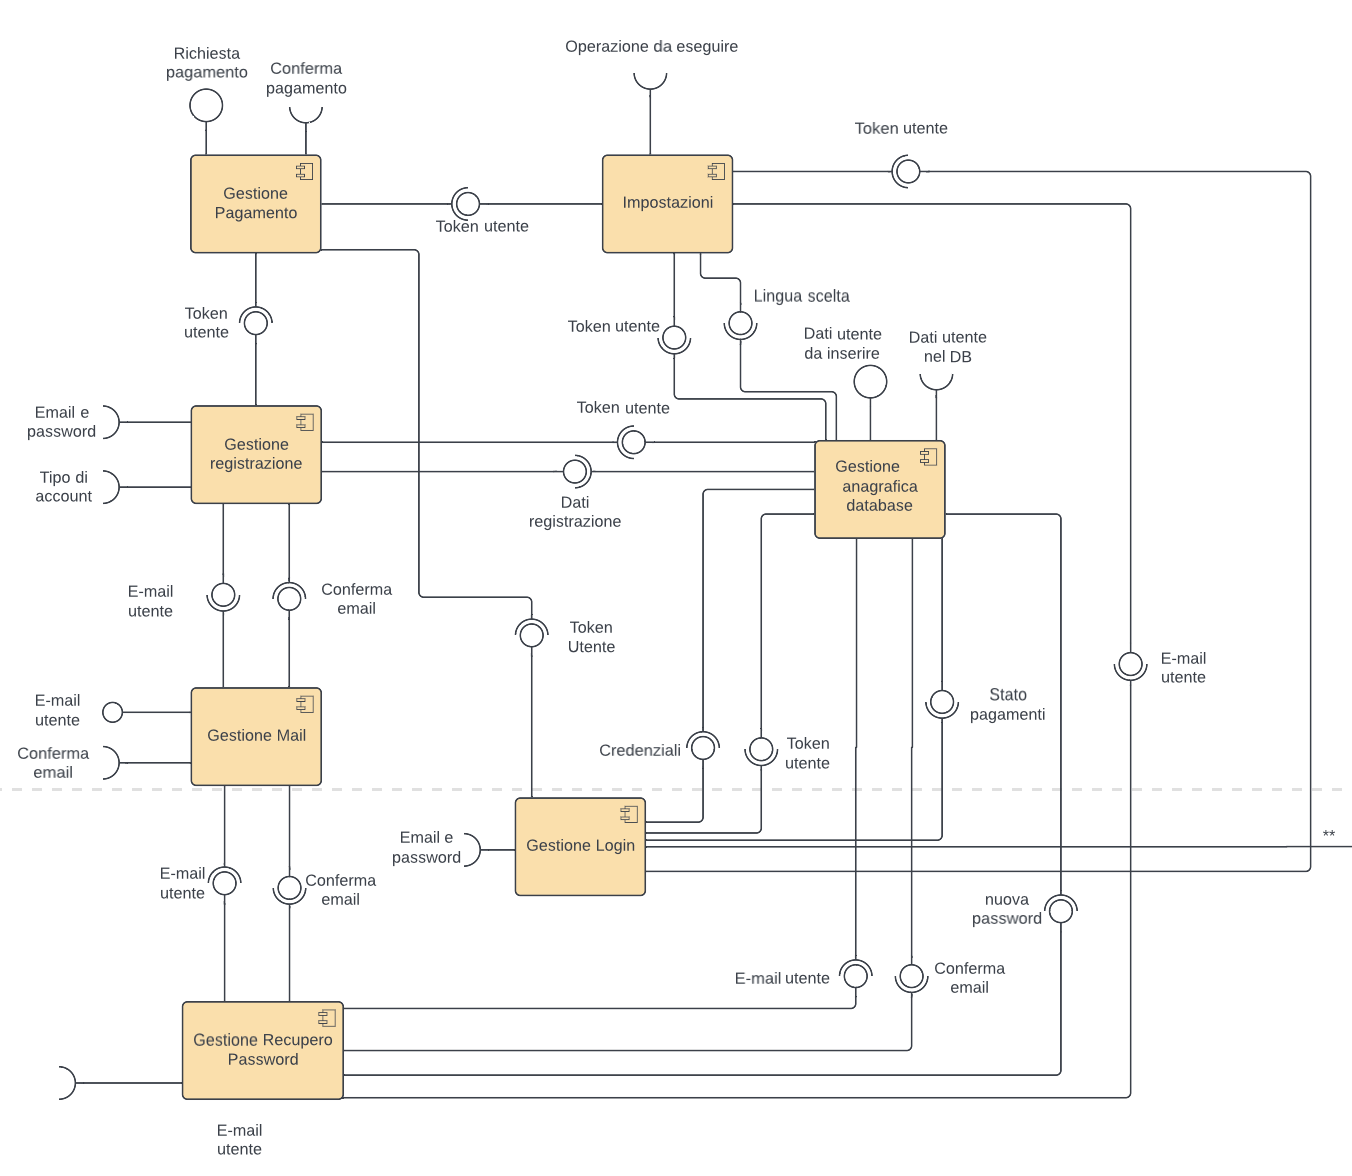
\includegraphics[width=\textwidth]{diagrams/component-1.png}
\end{figure}

\begin{figure}[htp]
    \centering
    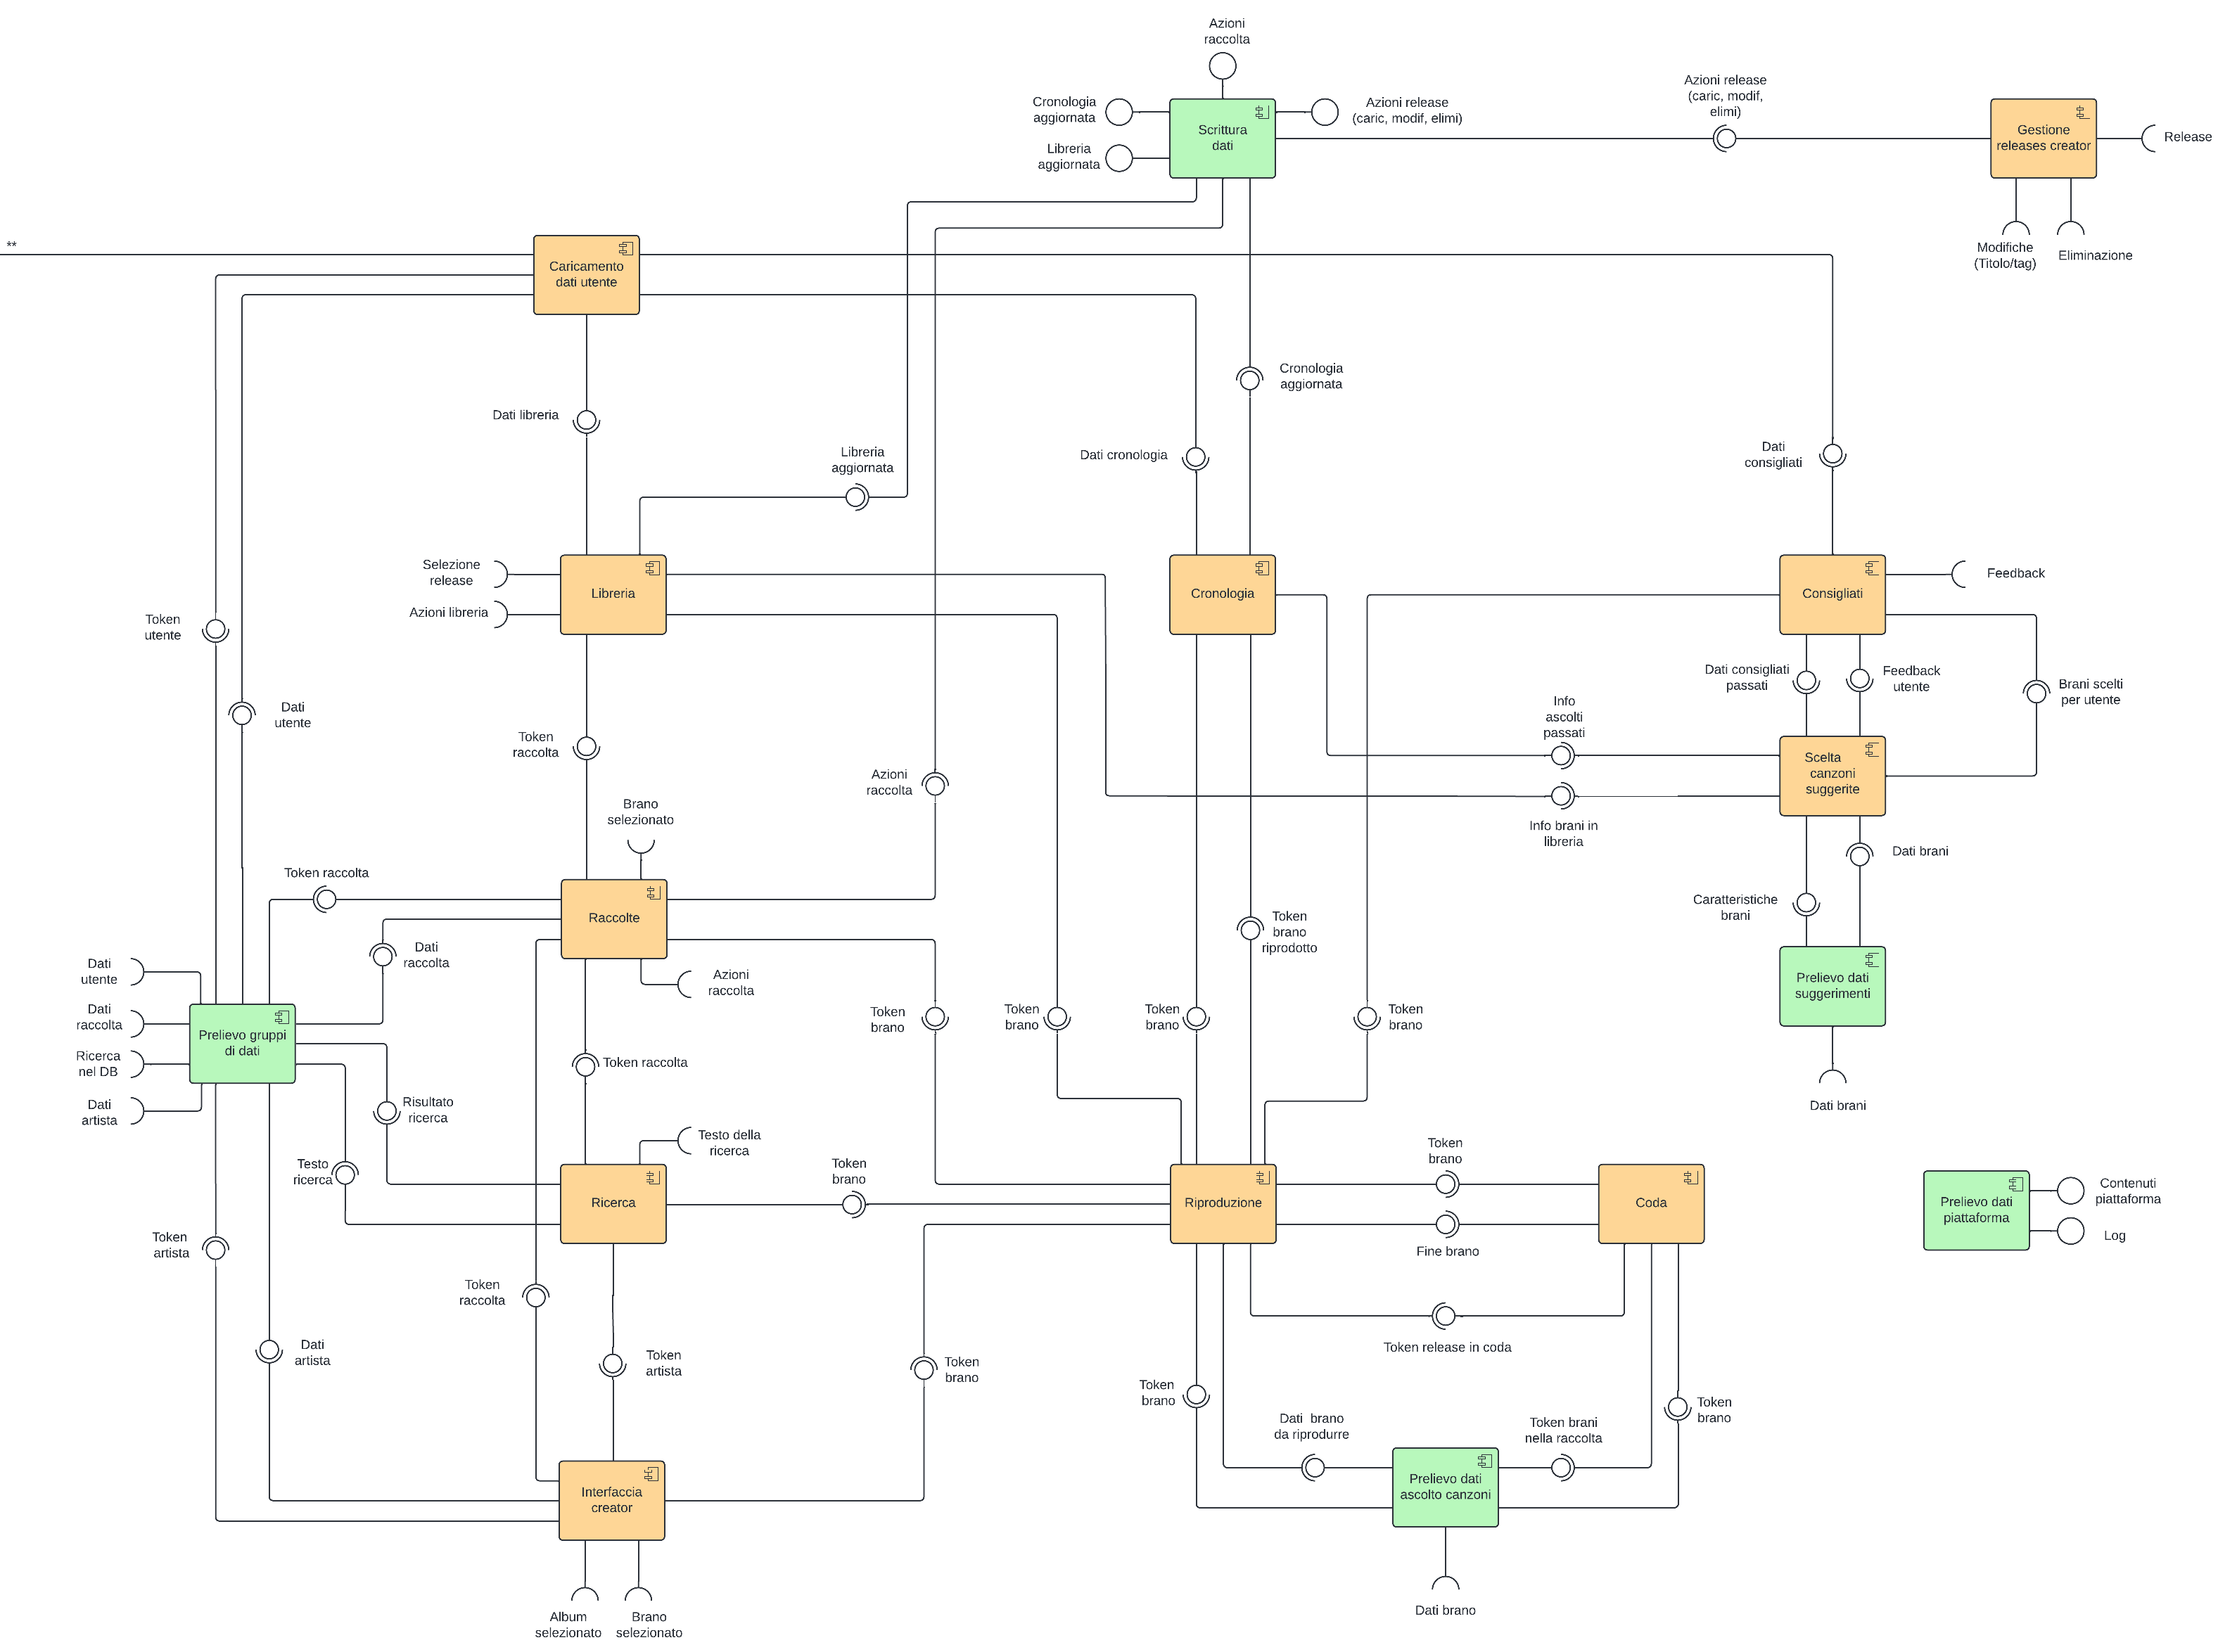
\includegraphics[angle=90,width=\textwidth]{diagrams/component-2.png}
\end{figure}

\end{document}